% =============================================================================
%  WCA-Bench: A Standardized Benchmark for Sports Analytics on
%            World Cube Association Competition Data
%
%  Compile with (XeLaTeX):
%      latexmk -xelatex main.tex
%  or manually:
%      xelatex main && bibtex main && xelatex main && xelatex main
%
%  arXiv-friendly: only common CTAN packages are used; no system-specific fonts.
% =============================================================================
\documentclass[11pt]{article}

% =============================================================================
%  preamble.tex -- shared packages and macros for WCA-Bench
%
%  Design constraints
%  ------------------
%   * Must compile with XeLaTeX (and also with pdfLaTeX as a fallback).
%   * Only widely available CTAN packages are used, so the source can be
%     uploaded to arXiv without a custom TeX Live installation.
%   * No fontawesome / academicons / todonotes / system-specific fonts.
%   * We deliberately avoid \usepackage{fontspec} and instead use the
%     Type-1 Times clone from the newtx bundle, which is available on every
%     TeX Live / MiKTeX installation and renders identically under XeLaTeX.
% =============================================================================

% --- encoding and fonts (Type-1, cross-platform, XeLaTeX-safe) --------------
\usepackage[T1]{fontenc}
\usepackage{newtxtext}
\usepackage{newtxmath}

% --- page geometry ----------------------------------------------------------
\usepackage[margin=1in]{geometry}
% Allow a little extra inter-word stretch so that long URLs / inline math do
% not force text into the margin.
\setlength{\emergencystretch}{3em}

% --- mathematics ------------------------------------------------------------
% NOTE: amssymb / amsfonts are intentionally omitted. They redefine \Bbbk,
% which newtxmath also provides, and loading both raises
% "Command \Bbbk already defined". newtxmath already supplies the AMS symbol
% fonts, and this document does not use any amssymb-only symbol.
\usepackage{amsmath}
\usepackage{mathtools}

% --- tables -----------------------------------------------------------------
\usepackage{booktabs}
\usepackage{multirow}
\usepackage{array}
\usepackage{tabularx}
\usepackage{threeparttable}
\usepackage{makecell}

% --- figures ----------------------------------------------------------------
\usepackage{graphicx}
\usepackage{xcolor}
\usepackage{caption}
\usepackage{subcaption}

% --- algorithms -------------------------------------------------------------
\usepackage{algorithm}
\usepackage{algpseudocode}

% --- typography and lists ---------------------------------------------------
\usepackage{microtype}
\usepackage{enumitem}
\setlist[itemize]{leftmargin=1.4em,topsep=2pt,itemsep=1pt}
\setlist[enumerate]{leftmargin=1.6em,topsep=2pt,itemsep=1pt}

% --- urls and references (loaded late) --------------------------------------
\usepackage{url}
\usepackage[numbers,sort&compress]{natbib}
\usepackage[hidelinks,breaklinks]{hyperref}

% --- captions ---------------------------------------------------------------
\captionsetup{font=small,labelfont=bf}

% --- custom colours ---------------------------------------------------------
\definecolor{wcablu}{HTML}{1F4E79}
\definecolor{wcared}{HTML}{B03A2E}
\definecolor{wcagrn}{HTML}{1E6B52}

% =============================================================================
%  Notation macros
% =============================================================================
\newcommand{\wca}{WCA}
\newcommand{\wcabench}{\textsc{WCA-Bench}}
\newcommand{\task}[1]{\textsf{T#1}}
\newcommand{\x}{\mathbf{x}}
\newcommand{\y}{y}
\newcommand{\asof}{\textsf{as\_of}}
\newcommand{\metric}{\mathcal{M}}
\newcommand{\loss}{\mathcal{L}}
\newcommand{\DNF}{\textsc{DNF}}
\newcommand{\DNS}{\textsc{DNS}}
% $\ensuremath{...}$ lets these macros be used in both text and math mode.
\newcommand{\kendall}{\ensuremath{\tau}}
\newcommand{\brier}{\ensuremath{B}}
\newcommand{\aucpr}{\ensuremath{\mathrm{AUC\text{-}PR}}}
\newcommand{\aucroc}{\ensuremath{\mathrm{AUC\text{-}ROC}}}
\newcommand{\maelog}{\ensuremath{\mathrm{MAE}_{\log}}}
\newcommand{\rmselog}{\ensuremath{\mathrm{RMSE}_{\log}}}
\newcommand{\ev}{\text{event}}

% "best seen so far", lower-is-better indicator used in result tables
\newcommand{\arrdown}{$\downarrow$}
\newcommand{\arrup}{$\uparrow$}

% =============================================================================
%  Algorithmic environment tweaks
% =============================================================================
\algrenewcommand\algorithmicrequire{\textbf{Input:}}
\algrenewcommand\algorithmicensure{\textbf{Output:}}

% =============================================================================
%  Small helpers
% =============================================================================
% tight column type for numeric tables
\newcolumntype{R}[1]{>{\raggedleft\arraybackslash}p{#1}}
\newcommand{\code}[1]{\texttt{#1}}

\endinput


% ------------------------------------------------------------------ metadata
\title{\textbf{WCA-Bench: A Standardized Benchmark for Sports Analytics\\ on World Cube Association Competition Data}}

\author{
  WCA-Bench Contributors\thanks{%
    Code released under the Apache-2.0 license. Competition data are owned and
    maintained by the World Cube Association and are redistributed only as
    derived, aggregate artifacts. Correspondence: \texttt{wcabench@example.org}.}
}

\date{\today}

% ------------------------------------------------------------------- document
\begin{document}

\maketitle

\begin{abstract}
We introduce \wcabench, the first standardized machine-learning benchmark built
on the complete public competition database of the World Cube Association
(\wca). Speedcubing is an unusual but instructive competitive setting: it is a
decades-long, globally distributed, individual-sport record of \emph{millions}
of timed attempts, governed by explicit rule systems (round formats,
``average of 5'' outlier trimming, multi-blind encodings, DNF/DNS status
codes) that generic time-series and tabular pipelines do not model. From a raw
export of \textbf{6{,}909{,}454 results}, \textbf{298{,}551 competitors} and
\textbf{18{,}708 competitions} we define a time split (train 2003--2022, val
2023--2024, test 2025--2026) and five tasks spanning regression, ranking,
imbalanced classification, extreme-value extrapolation and causal inference:
\task{1} result prediction, \task{2} placement prediction, \task{3} DNF
prediction, \task{4} human-limit estimation, and \task{5} skill transfer.
This paper makes four contributions: (i) a reproducible, columnar data
infrastructure with rule-aware decoding and a documented data card;
(ii) formal, metric-complete definitions for all five tasks together with
domain challenges; (iii) a leakage-safe rolling-window evaluation protocol
with frozen statistics, four-dimensional stratified reporting and a full
statistical-testing toolbox; and (iv) 21 reference baselines spanning six
methodological families---statistical, tree, deep, graph, Bayesian and
causal---with real measured numbers, for example \maelog{} $=0.164$
(single run) for tree-based result prediction, Kendall $\kendall=0.767$ for the
official psychology-sheet ranking baseline, and \aucpr{} $=0.373$ for
tree-based DNF prediction. We also release an honest account of where simple statistical
models remain competitive and where extrapolation and confounding make claims
unreliable.

\end{abstract}

\section{Introduction}
\label{sec:intro}

Predictive modelling of athletic performance is one of the oldest quantitative
pursuits in science, and the statistical literature on sports is enormous: it
ranges from rating systems for chess and ball games to forecasting individual
records in running and swimming. Yet most sports-analytics research is
conducted on bespoke, private or rapidly-changing datasets, which makes
results hard to compare. Each paper tends to choose its own data split, its own
preprocessing and its own metric, so two reported ``state-of-the-art'' numbers
are frequently not measuring the same thing. \wcabench{} addresses this
problem in a setting that has been almost entirely overlooked by the machine
learning community: competitive speedcubing, as recorded by the World Cube
Association (\wca).

\subsection{Motivation}
\label{sec:motivation}

Three problems motivate the benchmark.
\paragraph{Fragmented research.}
Existing work on \wca{} data is scattered across single tasks. Prior studies
have predicted competition placement with kernel density estimation, fitted
linear models to world-record trajectories, and estimated human limits with
Gaussian processes and extreme-value theory. Because these studies use
different splits, metrics and preprocessing, their conclusions cannot be
compared.
\paragraph{No standardized evaluation.}
The existing ``CubeBench''-style benchmarks target \emph{cube solving}: they
evaluate whether a language model or agent can plan a sequence of moves to
restore a scrambled cube. Those benchmarks are valuable, but they are
unrelated to the \wca's real competition records and cannot answer questions
such as ``which model predicts a competitor's time more accurately?'' or
``which method estimates the probability of a DNF more reliably?''. There is,
to our knowledge, no standardized benchmark for prediction and inference on
real speedcubing data.
\paragraph{Domain-specific structure is ignored.}
\wca{} data has unusual structure that general-purpose pipelines do not
handle: longitudinal competitor histories that span years; cross-event skill
transfer across 17 active events; round formats (\code{ao5}, \code{mo3},
best-of-3) that change how an average is computed; special status codes
($-1$ for \DNF{}, $-2$ for \DNS{}, $0$ for no result); and a compound encoding
for multi-blind results. A model that ignores the ``average of 5'' trimming
rule, for instance, will systematically miscalibrate both time and placement
predictions. We argue that these constraints deserve first-class treatment in
a benchmark rather than ad-hoc handling per paper.

\subsection{Contributions}
\label{sec:contributions}

We introduce \wcabench, a benchmark for prediction and inference on \wca{}
competition data. Our contributions are:

\begin{enumerate}
  \item \textbf{A reproducible data infrastructure.} A columnar
        (Parquet-based) pipeline that decodes every domain-specific value,
        including the \wca{} multi-blind compound encoding, round-format
        averaging with outlier trimming, and special status codes
        (Section~\ref{sec:dataset}). The pipeline is single-command
        reproducible and ships with a data card that documents provenance,
        scale, splits, biases and permitted/forbidden uses.

  \item \textbf{Five formalized tasks with domain-specific challenges.} We
        define \task{1} result prediction (regression), \task{2} placement
        prediction (ranking), \task{3} DNF prediction (imbalanced
        classification), \task{4} human-limit estimation (extreme-value
        extrapolation) and \task{5} skill-transfer analysis (causal
        inference). Each task is specified by an input/output/metric triple
        together with a baseline taxonomy and the domain challenges that make
        it non-trivial (Section~\ref{sec:tasks}).

  \item \textbf{A leakage-safe evaluation protocol and stratified
        reporting framework.} We specify a rolling-window protocol with
        frozen statistics, a four-dimensional stratification scheme (event,
        skill level, time slice, region) and a statistical-testing toolbox
        with effect sizes, designed so that small apparent gains are not
        over-claimed (Section~\ref{sec:protocol}).

  \item \textbf{21 reference baselines with real measured numbers.} We report
        actual baseline results on the official export
        (Section~\ref{sec:results}), covering six methodological
        families---statistical, tree, deep, graph, Bayesian and causal---with at
        least four baselines per task. For example, tree-based regression
        attains \maelog{} $=0.164$ on \task{1}; the \wca{} psychology sheet, a
        Plackett--Luce model and a kernel-density simulation all attain Kendall
        $\kendall=0.767$ on \task{2}; and tree-based classification attains
        \aucpr{} $=0.373$ on \task{3}. We deliberately do not claim
        state-of-the-art accuracy: the benchmark's scientific value lies in the
        standardized question, not in a new model.
\end{enumerate}

\subsection{Findings at a glance}
\label{sec:findings}

Because we release real numbers rather than hypothetical ones, the paper also
contains a first set of empirical observations, reported both for a single
seed and as a mean over three seeds (Section~\ref{sec:results-multiseed}).
Simple, well-specified models remain surprisingly competitive. On \task{2}, a
Plackett--Luce model, a kernel-density simulation and the official psychology
sheet produce \emph{identical} Kendall $\kendall=0.767$ to four decimals in the
seed-42 run ($0.8132\pm0.0342$ across seeds), whereas a graph neural network
reaches only $0.567$ ($0.7440\pm0.1258$). On \task{1}, a sequence model (LSTM,
\maelog{} $=1.044$, or $0.9436\pm0.0754$ across seeds) is much worse than
tree-based regression (\maelog{} $=0.164$, or $0.1055\pm0.0417$); and on
\task{3} the difference between the best tree model ($\aucpr{} 0.373$) and the
historical-rate prior ($\aucpr{} 0.359$) is \emph{not} statistically
significant ($p=0.749$, Cohen's $d=0.002$), while a Bayesian Beta--Binomial
model with no tree machinery is in fact best on average
($0.2938\pm0.0570$). Together these results suggest that, at this sample size,
rule-aware features combined with tree models dominate generic deep and graph
architectures. For human-limit estimation, the exponential-decay fit yields a
three-by-three limit of $3.74$ seconds, while the change-point model gives
$3.02$ seconds and the most stable method (Gaussian process plus extreme-value
theory) gives $3.29$ seconds---all well above the commonly cited domain anchor
of $2.37$ seconds, a concrete illustration of extrapolation risk. Finally, on
skill transfer, the number of ``identifiable'' event pairs falls monotonically
as identification assumptions tighten: Spearman correlation marks $413$, causal
forest $312$, instrumental variables $270$, and difference-in-differences only
$6$ ($2$ on average across seeds), quantifying how much the naive approach
over-claims. These observations are discussed in Section~\ref{sec:discussion}.

\subsection{Ethics and scope}
\label{sec:scope}

\wcabench{} is an evaluation benchmark, not a prediction product. It uses only
the publicly released \wca{} database export and never scrapes private data. We
explicitly forbid gambling, betting and any use that targets, ranks or
stigmatizes individual competitors, and we provide an opt-out mechanism
(Section~\ref{sec:limitations}). Out of scope are cube-solving/step-optimization
tasks (covered by cube-solving benchmarks such as \citep{cubebench, cube_bench_mllm}), LLM spatial-reasoning
evaluation, and live broadcast prediction systems.

\section{Related Work}
\label{sec:related}

\wcabench{} sits at the intersection of five research lines: \wca{} data
analysis, cube-solving benchmarks, sports analytics, time-series benchmarking,
and the methodology of dataset/benchmark papers.

\subsection{Speedcubing and World Cube Association data}
\label{sec:related-wca}

The \wca{} maintains the world's largest structured record of speedcubing
results, published as a versioned database export and governed by an explicit
rule book \citep{wca_export, wca_regs}. Prior work on this data has
concentrated on three narrow questions. Placement has been analysed with
dynamic paired-comparison and density-based rating models
\citep{glickman_rating}. World-record progression has been studied with
regression and saturating-curve models \citep{tatem_sprint, nevill_running}.
Human limits have been approached with extreme-value theory and saturating
curves \citep{evt_coles, nevill_running}. Each of these studies optimizes a
single task under its own protocol. Our contribution is not a better estimator
for any one of them but a common protocol under which all of them---and new
methods---can be evaluated and compared.

\subsection{Cube-solving benchmarks}
\label{sec:related-cubebench}

A parallel literature evaluates whether machines can \emph{solve} cubes. Early
work learned to solve the three-by-three cube with deep reinforcement learning
and search \citep{deepcubea} or with approximate policy iteration
\citep{mcaleer_cube}. More recently, a family of \emph{cube-reasoning
benchmarks} has emerged. CubeBench \citep{cubebench} builds a three-tiered
generative benchmark on the Rubik's cube to diagnose three cognitive challenges
that hinder LLM agents in physically grounded settings---spatial reasoning,
long-horizon state tracking, and active exploration under partial observations.
Cube Bench \citep{cube_bench_mllm} evaluates multimodal LLMs on five
spatial/sequential skills, from reconstructing cube faces from images to
multi-step planning and self-correction.

These benchmarks and ours are \emph{complementary rather than competing}: the
cube-reasoning benchmarks measure an agent's reasoning and planning ability on
\emph{synthetic} cube states, whereas \wcabench{} measures the predictive and
inferential ability of statistical and machine-learning models on \emph{real,
noisy, rule-governed competition records}. We therefore adopt a different
evaluation object (statistical/ML models rather than LLM/MLLM agents), a
different data source (real competitions rather than generated scrambles) and a
different task family (regression, ranking, classification, extreme-value
estimation and causal inference).

\subsection{Sports analytics}
\label{sec:related-sports}

Sports analytics has a long tradition of forecasting and rating. In
individual sports, performance-progression models for running and swimming
records are closely related to our \task{4} \citep{tatem_sprint,
nevill_running}. In team sports, ranking and outcome models built on
Bradley--Terry and Elo-style priors \citep{bradley_terry, elo} are the
ancestors of our \task{2} baselines, with the Plackett--Luce model
\citep{plackett_luce} providing the probabilistic ranking generalization we
use. In cricket, the Duckworth--Lewis method and its successors quantify how
context changes performance targets, an example of a \emph{rule-aware}
performance model. Injury- and fatigue-risk modelling in soccer and basketball
\citep{injury_prediction} resembles our \task{3} in that it predicts rare,
consequential events from longitudinal records. Our benchmark borrows the
discipline of these fields---time-aware splits, calibration, effect sizes---and
packages it for a new domain.

\subsection{Time-series and tabular benchmarking}
\label{sec:related-ts}

Standardized forecasting competitions and corpora have shaped evaluation
practice, notably the M-competitions and the M5 accuracy competition
\citep{m5_competition}, the Monash Time Series Forecasting Archive
\citep{monash_tsf} and the GluonTS toolkit \citep{gluonts}. These resources
established the norms we follow: a fixed, frozen test window; explicit
avoidance of future leakage; stratified reporting; and public leaderboards,
building on standard forecasting methodology \citep{hyndman_fpp3}.
\wcabench{} differs in that its series are indexed by irregular competition
calendars rather than regular timestamps, and in that the prediction targets
are governed by formal round rules. For online/incremental learning, the
prequential (test-then-train) evaluation tradition \citep{prequential} is the
closest methodological relative of our rolling-window protocol.

\subsection{Extreme-value estimation and human limits}
\label{sec:related-evt}

Estimating an unobservable performance ceiling is an extrapolation problem.
Extreme-value theory provides the asymptotic machinery for tail behaviour
\citep{evt_coles, pickands}, while saturating-curve models are the pragmatic
choice in sports \citep{nevill_running, tatem_sprint}. Bayesian hierarchical models let
sports with scarce data borrow strength from a population of similar events
\citep{bayesian_hierarchical}. Our \task{4} benchmark exposes exactly this
tension: recurring events have dense histories, while emerging or discontinued
events may have fewer than fifty world-record points, forcing explicit
modelling choices that we make comparable across methods.

\subsection{Causal inference in observational sports data}
\label{sec:related-causal}

Our \task{5} formalizes a question---does practising event $A$ causally improve
event $B$?---that is deceptively hard because participation is self-selected.
Difference-in-differences \citep{did}, instrumental variables \citep{iv},
regression discontinuity, and causal forests \citep{causal_forest} are the
standard tools, each resting on a different identification assumption. This
mirrors causal inference in economics and epidemiology, where the honest
reporting of assumptions and sensitivity analyses has become standard
\citep{sensitivity_analysis}. We deliberately include a naive correlational
baseline to make the gap between association and causation measurable.

\subsection{Benchmark and dataset methodology}
\label{sec:related-methodology}

Our documentation and reporting follow the datasheet \citep{datasheets} and
model-card \citep{model_cards} traditions, which argue that datasets and
models must document provenance, composition, recommended uses and limitations.
We adopt the NeurIPS Datasets and Benchmarks evaluation philosophy
\citep{neurips_dnb} by requiring stratified results, calibration and effect
sizes rather than a single headline number. Our leakage-aware protocol echoes
broader warnings about spurious leakage in machine learning evaluation
\citep{leakage_kaufman}.

\paragraph{Deep and graph methods in this setting.} Our measured multi-seed
results speak directly to the above lines of work
(Section~\ref{sec:results-multiseed}): on \task{1} a sequence model
(\maelog{} $0.9436\pm0.0754$) is roughly nine times worse than tree boosting
($0.1055\pm0.0417$), and on \task{2} a graph neural network
($\kendall=0.7440\pm0.1258$) trails a simple domain ranking
($0.8132\pm0.0342$). In rule-governed longitudinal sports records, domain-aware
features currently appear to matter more than generic deep or graph
architectures.

\section{The \wcabench{} Dataset}
\label{sec:dataset}

This section documents the data source, scale, schema, domain-specific
decoding rules, temporal splits and known biases. We follow the datasheet
convention \citep{datasheets}: anything a downstream user needs in order to
judge whether the benchmark is appropriate for their question is stated here
or in the accompanying data card.

\subsection{Source and provenance}
\label{sec:data-source}

All data originate from the official \wca{} public database export
\citep{wca_export}, a versioned, freely downloadable snapshot of every
sanctioned competition. We use the \code{Results Export} format
\textbf{v2.0.2} (snake-case column names, including the \code{result\_attempts}
table) with an export date of 2026-09-21. No private, scraped or synthetic data
are used for headline results; a synthetic generator is provided separately for
offline continuous-integration runs, and any result computed on synthetic data
is labelled as such. The code is released under Apache-2.0; the data remain
the property of the \wca{} and are redistributed only as derived aggregates.

\subsection{Scale}
\label{sec:data-scale}

Table~\ref{tab:scale} summarizes the scale of the built artifacts. The raw
export contains millions of individual timed attempts, which is what makes the
benchmark statistically rich and simultaneously computationally demanding.

These counts are \textbf{this benchmark's snapshot statistics}, not figures
published by \wca{}: they are the exact row counts of the pinned export
snapshot and are reproducible from \code{data/processed/manifest.json} and the
reconciliation report.\footnote{Snapshot metadata: export format version
\textbf{v2.0.2}; export date \textbf{2026-09-21} (readme and
\code{metadata.json}); the official export enumerates 14 tables but publishes
\emph{no} per-table row counts.} The official \wca{} export pages expose only
the format version (v2.0.2), the export date and download sizes (the SQL
archive is $390{,}136{,}209$~bytes and the TSV archive $377{,}258{,}709$~bytes,
as of 2026-09-21). We therefore report both the snapshot counts and the
official qualitative scale, and we caution that the \wca{} database grows
continuously, so a newer export will not match these numbers exactly
(Section~\ref{sec:limitations}).

\begin{table}[t]
  \centering
  \small
  \begin{threeparttable}
  \caption{Scale of the \wcabench{} data artifacts. All row counts are
  \emph{snapshot statistics} of this benchmark's pinned export
  (v2.0.2, export date 2026-09-21).}
  \label{tab:scale}
  \begin{tabular}{lr}
    \toprule
    Quantity & Value \\
    \midrule
    Results (person--event--round records) & 6{,}909{,}454 \\
    Competitors (\code{persons}) & 298{,}551 \\
    Competitions (\code{competitions}) & 18{,}708 \\
    Single attempts (\code{result\_attempts}) & 31{,}847{,}257 \\
    Scramble rows (\code{scrambles}) & 3{,}186{,}380 \\
    Events (active + discontinued) & 22 \\
    \midrule
    Train split (2003--2022) & 3{,}211{,}294 \\
    Validation split (2023--2024) & 1{,}978{,}851 \\
    Test split (2025--2026) & 1{,}719{,}290 \\
    \midrule
    Global attempt-level \DNF{} rate & 3.18\% \\
    Frozen person--event statistics & 612{,}224 \\
    \bottomrule
  \end{tabular}
  \begin{tablenotes}\footnotesize
    \item ``Frozen person--event statistics'' counts the per-(person, event)
          historical summaries computed on the training window and held fixed
          for the whole test window (Section~\ref{sec:protocol}).
  \end{tablenotes}
  \end{threeparttable}
\end{table}

The 21 events comprise the 17 currently sanctioned events (three-by-three
through seven-by-seven, one-handed, blindfolded, fewest-moves, multi-blind,
clock, megaminx, pyraminx, skewb, square-1) plus four historical or
discontinued events (three-by-three feet, magic, master magic and old-style
multi-blind). Event coverage is highly imbalanced: three-by-three dominates by
an order of magnitude, whereas multi-blind, four-blind and five-blind have
comparatively few records. This imbalance is the primary reason for the
stratified reporting in Section~\ref{sec:protocol}.

\subsection{Schema}
\label{sec:data-schema}

The benchmark uses the following relational tables, joined through the keys
shown in Table~\ref{tab:schema}.

\begin{table}[t]
  \centering
  \small
  \begin{threeparttable}
  \caption{Core tables and the joins that define the benchmark's relational
  view.}
  \label{tab:schema}
  \begin{tabular}{@{}lll@{}}
    \toprule
    Table & Key fields & Role in the benchmark \\
    \midrule
    \code{persons} & \code{wca\_id}, name, country, gender & competitor identity \\
    \code{competitions} & \code{id}, date, city, coordinates & temporal anchor \\
    \code{results} & (person, competition, event, round) & labels: best, average, pos \\
    \code{result\_attempts} & result key, attempt number & per-attempt values \\
    \code{scrambles} & round key, group & scramble sequences \\
    \code{events} / \code{formats} / \code{round\_types} & id & scoring semantics \\
    \code{countries} / \code{continents} & iso2 & regional stratification \\
    \code{championships} & competition id & optional competition context \\
    \bottomrule
  \end{tabular}
  \begin{tablenotes}\footnotesize
    \item In v2.0.2 the \code{result\_attempts} table no longer carries
          \code{id}/\code{created\_at}/\code{updated\_at}; pipelines must not
          depend on them.
  \end{tablenotes}
  \end{threeparttable}
\end{table}

\subsection{Domain-specific decoding}
\label{sec:data-decoding}

The decisive feature of \wca{} data is that the meaning of a stored integer
depends on the event's \code{format}. We state the decoding rules explicitly,
because mishandling them corrupts every downstream task.

\paragraph{Timed and count-based values.}
For \code{time} events a positive value is a number of centiseconds
(\code{8653} $= 1{:}26.53$). For the fewest-moves event (\code{number}) a
positive value is a raw move count, and averages are stored as $100\times$ the
mean. Negative and zero sentinels encode status: $-1$ means \DNF{} (did not
finish), $-2$ means \DNS{} (did not start), and $0$ means ``no result''.
\DNF{} attempts participate in \DNF{}-rate statistics but never in an average;
\DNS{} is normally excluded from training; $0$ is treated as missing.

\paragraph{Multi-blind compound encoding.}
The multi-blind event (\code{333mbf}) stores a composite integer whose ten
digits pack the number of solved cubes, the number attempted and the elapsed
time into one value. Two generations exist, distinguished by the leading digit.
Algorithm~\ref{alg:multi} gives the decoder we implement (and its exact
inverse, used for round-trip testing).

\begin{algorithm}[t]
\caption{Decoding of the \wca{} multi-blind compound value.}
\label{alg:multi}
\begin{algorithmic}[1]
\Require positive integer $v$ (10-digit, zero-padded string $s$)
\Ensure solved, attempted, seconds
\State $s \gets \mathrm{zfill}(\mathrm{str}(v), 10)$
\If{$s_0 = \texttt{1}$} \Comment{old format \texttt{1SSAATTTTT}}
    \State $SS \gets \mathrm{int}(s_{1:3})$, $AA \gets \mathrm{int}(s_{3:5})$
    \State solved $\gets 99 - SS$
    \State attempted $\gets AA$
    \State seconds $\gets \mathrm{int}(s_{5:10})$
    \State missed $\gets$ attempted $-$ solved \Comment{requires missed $\ge 0$}
\ElsIf{$s_0 = \texttt{0}$} \Comment{new format \texttt{0DDTTTTTMM}}
    \State $DD \gets \mathrm{int}(s_{1:3})$, $MM \gets \mathrm{int}(s_{8:10})$
    \State seconds $\gets \mathrm{int}(s_{3:8})$
    \State difference $\gets 99 - DD$
    \State solved $\gets$ difference $+$ missed, where missed $\gets MM$
    \State attempted $\gets$ solved $+$ missed
\Else
    \State \textbf{error} unknown version digit
\EndIf
\end{algorithmic}
\end{algorithm}

The stored double-blind score used for ranking is the lower-is-better surrogate
$(100-\text{solved})\times 10^6 + \text{seconds} + \text{missed}$, which
preserves the \wca{} ordering while remaining a single scalar per attempt.

\paragraph{Round-format normalization.}
Several round formats require averaging with outlier trimming. For
\emph{average of 5} (\code{ao5}) an attempt set of five is sorted, the best and
worst attempts are discarded, and the remaining three are averaged; if two or
more attempts are \DNF{}, the whole round is \DNF{}. For \emph{mean of 3}
(\code{mo3}) all three attempts are averaged, and any \DNF{} makes the round
\DNF{}. We reconstruct each round's average from \code{result\_attempts} and
check it against the official \code{results.average}; the consistency rate is
tracked as a data-quality gate. This trimming rule matters because a single
\DNF{} in \code{ao5} is usually absorbed as the discarded ``worst'' attempt,
so the marginal effect of one \DNF{} is small, while a second \DNF{} collapses
the round---a discontinuity that models must represent explicitly rather than
average away.

\paragraph{Scrambles.}
Multi-blind scrambles consist of several newline-separated three-by-three
scrambles; in the TSV export newlines are replaced by the pipe character
(\code{|}). The pipeline splits on \code{|} (or newline), trims, and validates
the resulting sequence length against the event.

\subsection{Temporal splits}
\label{sec:data-splits}

We adopt a strict temporal split rather than a random one. Random splits leak
future information, because adjacent competitions of the same competitor are
strongly correlated; a temporal split instead mirrors the real deployment
setting of predicting the future from the past.

\begin{table}[t]
  \centering
  \small
  \begin{threeparttable}
  \caption{Temporal split of \wcabench{}. The test window is fixed so that the
  main leaderboard remains comparable as new data arrive.}
  \label{tab:splits}
  \begin{tabular}{llr}
    \toprule
    Split & Window & Records \\
    \midrule
    Train & 2003--2022 & 3{,}211{,}294 \\
    Validation & 2023--2024 & 1{,}978{,}851 \\
    Test (frozen) & 2025--2026 & 1{,}719{,}290 \\
    \quad Test-A & 2025 H1 & --- \\
    \quad Test-B & 2025 H2 & --- \\
    \quad Test-C & 2026 H1 & --- \\
    \bottomrule
  \end{tabular}
  \begin{tablenotes}\footnotesize
    \item Per-slice record counts are reported at evaluation time and depend on
          the sampled test set; the sub-slices are used for temporal-robustness
          stratification.
  \end{tablenotes}
  \end{threeparttable}
\end{table}

Each competitor additionally retains a complete, time-ordered competition
history, enabling longitudinal analysis. Because the \wca{} database keeps
growing, the main leaderboard is always computed on the fixed 2025--2026 test
window; later competitions are published as a separate \emph{extended test
set}, following the convention of time-series benchmarks.

\subsection{Known biases}
\label{sec:data-biases}

We list the biases that a responsible user must keep in mind; the same list
appears in the data card.
\begin{itemize}
  \item \textbf{Event imbalance.} Three-by-three records vastly outnumber
        multi-blind, four-blind and five-blind records. Unstratified averages
        are therefore dominated by three-by-three.
  \item \textbf{Regional imbalance.} Access to competitions differs sharply by
        country and continent, so cross-regional generalization claims are
        weak by construction.
  \item \textbf{Class imbalance.} \DNF{} is rare (3.18\% of attempts overall)
        and extremely uneven across events; blindfolded and multi-blind events
        have far higher failure rates.
  \item \textbf{Non-stationarity.} Hardware changes (for example magnetic
        cubes), rule changes and training-method shifts make the time series
        non-stationary; a model fitted on 2003--2022 does not face the same
        distribution in 2025--2026.
  \item \textbf{Self-selection.} Participation in an event is a choice, so
        skill-transfer estimates are confounded; simple correlation
        systematically overstates transfer (Section~\ref{sec:tasks}).
  \item \textbf{Cold start.} Competitors whose first appearance falls inside
        the test window have no usable history; they are flagged and reported
        separately rather than silently merged into the main metric.
\end{itemize}

\section{Tasks}
\label{sec:tasks}

\wcabench{} defines five tasks that span a continuous difficulty spectrum from
supervised regression to causal inference. Every task is specified by the same
five elements---formal definition, inputs and outputs, metrics, baselines and
domain challenges---and every task is exposed through a single interface so
that one evaluation code path scores all models. We use the notation
$\x$ for the model input, $\y$ for the target and $\metric$ for the metric
set.

\paragraph{The common interface.}
All tasks implement
\begin{center}\small
\code{split()} $\to$ temporal view;\quad
\code{featurize(as\_of)} $\to$ features;\quad
\code{metrics()} $\to$ metric list;\quad
\code{baseline()} $\to$ registered baselines;\quad
\code{evaluate(model)} $\to$ report.
\end{center}
The \asof{} argument is \emph{mandatory} in the feature-construction signature.
This is a design decision: leakage prevention is a type-level obligation, not
an afterthought. Baselines are organized into three tiers---trivial, domain and
methodological---and the methodological tier spans six families (statistical,
tree, deep, graph, Bayesian and causal), so that a reader can see how much is
gained over a meaningful reference point rather than over an arbitrary zero, and
can compare methodological families directly against one another.

% -----------------------------------------------------------------------------
\subsection{\task{1}: Result Prediction (Regression)}
\label{sec:task1}

\paragraph{Definition.}
Given a competitor's pre-competition history, predict the \code{best} and
\code{average} result the competitor will achieve in a specific competition,
event and round. Formally, let
$\y = f_\theta(\x)$ where
$\x = (\x^{\text{seq}}, \x^{\text{static}}, \asof)$ and
$\y = (\hat{b}, \hat{a}, \hat{\sigma}^2)$ denote predicted best, average and
predictive variance.

\paragraph{Inputs.}
Identity fields (competitor, competition, event, round type); the historical
result sequence of the last $N$ attempts; static features (age, gender,
nationality, total competition count); and the enforced decision timestamp
\asof{}.

\paragraph{Outputs.}
Continuous best and average predictions (average only where the format
supports it) and distributional parameters for interval estimation.

\paragraph{Metrics.}
Because events differ enormously in magnitude, we compute errors in the
\emph{log domain}: \maelog{} (primary) and \rmselog{} (secondary), plus
prediction-interval coverage (a calibration metric). Reporting is stratified by
competitor skill level.

\paragraph{Baselines.}
Trivial: the historical mean of the last 25 attempts. Domain/statistical:
linear extrapolation of recent results, and kernel density estimation with
bootstrap round simulation. Methodological: sequence models such as
LSTM/Transformer encoders, and gradient-boosted regression on log-transformed
targets.

\paragraph{Domain challenges.}
Performance is non-stationary: training-method improvements, injuries and
hardware changes can produce step changes in a competitor's results.
Between-event variance differs by orders of magnitude (seconds for
three-by-three, minutes for seven-by-seven, integer move counts for
fewest-moves), so event-specific normalization is essential.

% -----------------------------------------------------------------------------
\subsection{\task{2}: Placement Prediction (Ranking)}
\label{sec:task2}

\paragraph{Definition.}
Given the histories of \emph{all} competitors entered in a round, predict the
final ordering. For a round with competitor set $\mathcal{P}$, learn a scoring
function $s_\phi(\x_i)$ and output a permutation
$\hat{\pi} = \mathrm{argsort}_{i \in \mathcal{P}}(-s_\phi(\x_i))$ together with
a distribution $P(\mathrm{rank}_i = k)$ and a podium probability
$P(\mathrm{rank}_i \le 3)$.

\paragraph{Inputs.}
Competition context (competition, event, round type); history features for
every entered competitor; the enforced \asof{} timestamp.

\paragraph{Outputs.}
Predicted integer ranks, rank distributions and podium probabilities.

\paragraph{Metrics.}
Kendall's $\kendall$ rank correlation (primary), top-3 overlap with the true
podium, the Brier score of the podium probabilities, and a direct comparison
against the official \wca{} psychology sheet.

\paragraph{Baselines.}
Domain: the \wca{} \emph{psychology sheet}, which ranks competitors by their
best historical \code{ao5} and ignores variance or consistency---a strong,
practically relevant reference. Statistical: kernel-density Monte Carlo rank
simulation and the Plackett--Luce model \citep{plackett_luce}, which assigns
each competitor a latent strength and defines a distribution over orderings.
Methodological: a graph neural network over a competitor--competition
heterogeneous graph that models head-to-head interactions.

\paragraph{Domain challenges.}
The central difficulty is interaction: the same competitor may perform
differently against different fields, so the model must capture relative, not
merely absolute, strength. Round rules interact with \DNF{}: one \DNF{} is
usually discarded as the worst \code{ao5} attempt, but two \DNF{}s collapse the
round and the ranking. Round sizes vary from a handful to several hundred
competitors, which makes fixed-length ranking architectures awkward.

% -----------------------------------------------------------------------------
\subsection{\task{3}: DNF Prediction (Imbalanced Classification)}
\label{sec:task3}

\paragraph{Definition.}
Given the attempts a competitor has already completed in a round and the
number remaining, predict the probability that a subsequent attempt is a
\DNF{}. Formally, with partial sequence
$\x = (x_1, \dots, x_{k})$ and round context $c$ (format, attempts left),
estimate $P(\text{DNF} \mid \x, c)$ and the whole-round probability
$P(\text{round DNF})$.

\paragraph{Inputs.}
Competitor identity; the completed attempt values (including \DNF{} markers);
round format and remaining attempts; the competitor's historical \DNF{} rate;
the enforced \asof{} timestamp.

\paragraph{Outputs.}
A per-attempt \DNF{} probability and a whole-round \DNF{} probability.

\paragraph{Metrics.}
\aucroc{} and \aucpr{} (with the latter emphasized under imbalance), F1, the
Matthews correlation coefficient (MCC), and a reliability diagram for
calibration. Because \aucroc{} flatters models when positives are rare, we
require \aucpr{} and MCC alongside a random/global-rate reference. We also
report a \emph{hard subset} on which the competitor's historical \DNF{} rate
lies in $[0.1, 0.3]$, to preserve discriminative power against saturation.

\paragraph{Baselines.}
Trivial/domain: the competitor's historical \DNF{} rate. Statistical:
logistic regression on completed-attempt mean and variance, and a Bayesian
hierarchical model with a Beta prior for shrinkage. Methodological: random
forest / gradient boosting over competitor and round-context features.

\paragraph{Domain challenges.}
\DNF{} is rare and unevenly distributed: blindfolded and multi-blind events
fail far more often, while three-by-three is stable, and fewest-moves has its
own timeout/violation failure mode. \DNF{} occurrence is also
sequence-dependent: after a failure a competitor may become more conservative
(reducing risk) or may lose composure (increasing it). Finally, risk is
rule-dependent---after one \DNF{} in \code{ao5} the tolerance for another
failure is zero.

% -----------------------------------------------------------------------------
\subsection{\task{4}: Human-Limit Estimation (Extreme-Value Extrapolation)}
\label{sec:task4}

\paragraph{Definition.}
From each event's historical world-record series
$\{(t_i, y_i)\}$ estimate the theoretical performance ceiling $L$ and the
year at which it is expected to be approached. Employ the saturating model
\begin{equation}
  y(t) = L + (y_0 - L)\,\exp\!\big(-\lambda\, g(t)\big) + \varepsilon(t),
  \label{eq:limit}
\end{equation}
where $L$ is the limit, $g(t)$ is a technological-progress function and
$\varepsilon$ is noise, and infer the posterior $p(L, \lambda, \text{params}
\mid \text{data})$.

\paragraph{Inputs.}
The world-record series per event (date, value), plus event-level features
(mean, variance, history length).

\paragraph{Outputs.}
A point estimate and posterior for $L$, the predictive interval, and a
convergence-year estimate with an interval.

\paragraph{Metrics.}
There is no observable ground truth for a limit, so evaluation relies on
(a) stability of the estimate under leave-one-out refitting, (b) empirical
coverage of the predictive intervals, and (c) consistency with established
domain knowledge. As an anchor, the speedcubing community estimates the
three-by-three limit near $2.37$ seconds with convergence around 2036.

\paragraph{Baselines.}
Statistical: the exponential-decay model of Equation~\ref{eq:limit}.
Methodological: Gaussian-process regression combined with extreme-value theory
\citep{evt_coles}; a Bayesian hierarchical extreme-value model
that treats per-event limits as draws from a hyper-distribution
\citep{bayesian_hierarchical}; and change-point detection that identifies
structural breaks in the rate of improvement.

\paragraph{Domain challenges.}
The dominant risk is extrapolation: historical data cannot anticipate a future
jump caused by new hardware or training regimes. Data density varies wildly;
three-by-three has 23 years of dense data, whereas some events provide fewer
than fifty record points and demand strong priors or hierarchical borrowing.
Finally, the target is unobservable, so validation must be indirect.

% -----------------------------------------------------------------------------
\subsection{\task{5}: Skill Transfer (Causal Inference)}
\label{sec:task5}

\paragraph{Definition.}
Quantify how an improvement in one event causally affects performance in
another. For each ordered event pair $(A, B)$ estimate the causal effect
$\theta_{A \to B}$ and assemble a $17 \times 17$ transfer matrix with
confidence intervals.

\paragraph{Inputs.}
Competitors' multi-event records (timestamp, event, result) and the time at
which each competitor first participated in each event.

\paragraph{Outputs.}
A transfer matrix $\Theta = [\theta_{A \to B}]$ and interval estimates, with an
explicit identifiability flag for pairs that cannot be estimated reliably.

\paragraph{Metrics.}
Point-estimate accuracy against held-out data, robustness of the estimate
across subsamples, and agreement with domain-expert judgement. Because a
ground-truth effect is unavailable, we additionally report the
\emph{number of identifiable event pairs}.

\paragraph{Baselines.}
Correlational: Pearson/Spearman correlation between event performances---the
naive approach that ignores confounding. Causal: difference-in-differences
(DID) \citep{did} treating first participation in event $A$ as treatment;
instrumental variables (IV) \citep{iv} using the first domestic hosting of an
event as an instrument; and a causal forest \citep{causal_forest} for
heterogeneous treatment effects.

\paragraph{Domain challenges.}
Confounding is severe: talent and training effort raise performance in all
events simultaneously, producing spurious positive transfer. Participation
order is non-random---competitors who are good at event $A$ may take up event
$B$ earlier---which induces self-selection bias. Finally, many event pairs have
very few common competitors, so effects are poorly identified and the benchmark
requires an explicit ``not identifiable'' label rather than a forced estimate.

\section{Evaluation Protocol}
\label{sec:protocol}

A benchmark is only as trustworthy as its evaluation protocol. \wcabench{}
rests on four pillars: leakage prevention, stratified reporting, statistical
rigour, and reproducibility. Empirical rigour of this kind is increasingly
recognized as essential for progress \citep{sculley_rigor}. This section
specifies each pillar in turn.

\subsection{Leakage prevention}
\label{sec:protocol-leakage}

\wcabench{} uses a rolling-window evaluation that simulates deployment: for
every test competition, only data that existed \emph{before} that competition
may influence a prediction. Formally, for a target competition with date $d$,
the admissible information set is
$\mathcal{F}_d = \{\, r : \mathrm{date}(r) < d \,\}$, and no record at or after
$d$---including other competitors' results in the same round---may be used.

Three mechanisms enforce this. First, every feature function must accept an
explicit \asof{} timestamp; a feature that cannot be evaluated ``as of'' a
moment is not admissible. Feature caches are keyed by \asof{} so results cannot
be silently reused across time. Second, a testing utility
\code{assert\_no\_leakage(features, target\_date)} asserts that no feature
depends on a record dated at or after the target. Third, benchmark statistics
are frozen, as described next.

\subsection{Frozen statistics}
\label{sec:protocol-frozen}

Statistics that would otherwise drift as the test window advances are computed
once from the training window and held fixed for the entire test period.
Table~\ref{tab:frozen} lists them. Freezing is essential: if, for example,
``current world record'' were recomputed per test competition, a model could
benefit from information that a real deployment would not have at the decision
moment. The export contains \textbf{612{,}224} frozen person--event
statistics, each computed on the training split only.

\begin{table}[t]
  \centering
  \small
  \begin{threeparttable}
  \caption{Statistics frozen from the training window and reused for the whole
  test window.}
  \label{tab:frozen}
  \begin{tabular}{@{}lll@{}}
    \toprule
    Statistic & Computed from & Frozen for \\
    \midrule
    Competitor historical mean / variance & training ($\le 2022$) & whole test window \\
    Event world record & training & whole test window \\
    Event reference distribution & training & whole test window \\
    Skill-level percentile thresholds & training & whole test window \\
    \bottomrule
  \end{tabular}
  \end{threeparttable}
\end{table}

\subsection{Rolling-window algorithm}
\label{sec:protocol-algorithm}

Algorithm~\ref{alg:rolling} gives the protocol in pseudocode. Test competitions
are processed in chronological order; features are built from the frozen
statistics and the running history, a leakage assertion is checked, and
per-competition reports are aggregated at the end.

\begin{algorithm}[t]
\caption{Rolling-window evaluation with frozen statistics.}
\label{alg:rolling}
\begin{algorithmic}[1]
\Require model $f$, test competitions $C$, frozen statistics $F$
\Ensure aggregated report
\State $R \gets [\,]$
\State $C \gets \mathrm{sort}(C, \text{key} = \text{date})$ \Comment{chronological}
\ForAll{$c \in C$}
    \State $\x \gets \textsc{Featurize}(\asof = c.\text{date}, F)$
    \State \textbf{assert} \Call{NoLeakage}{$\x$, $c.\text{date}$}
    \State $\hat{\y} \gets f.\mathrm{predict}(\x)$
    \State $R.\mathrm{append}\big(\textsc{Evaluate}(\hat{\y}, c.\text{truth})\big)$
\EndFor
\State \Return \Call{Aggregate}{$R$}
\end{algorithmic}
\end{algorithm}

\subsection{Four-dimensional stratification}
\label{sec:protocol-stratification}

Aggregate metrics can be dominated by a single large subgroup. To prevent
conclusions from being masked, \wcabench{} mandates stratified reports along
four dimensions, summarized in Table~\ref{tab:strat}. All four are emitted
together with confidence intervals, so a reader can see whether a headline gain
holds within important subgroups.

\begin{table}[t]
  \centering
  \small
  \begin{threeparttable}
  \caption{The four stratification dimensions required for every task.}
  \label{tab:strat}
  \begin{tabular}{@{}lll@{}}
    \toprule
    Dimension & Groups & Rationale \\
    \midrule
    Event & speed-solving / variant / blind / other & data volume differs by orders of magnitude \\
    Skill level & novice (0--25\%), intermediate (25--75\%), & behaviour and stability differ by level \\
                & advanced (75--95\%), elite ($>$95\%) & \\
    Time slice & Test-A / Test-B / Test-C & temporal robustness \\
    Region & Asia, Europe, North America, & cross-regional generalization \\
           & South America, Oceania, Africa & \\
    \bottomrule
  \end{tabular}
  \end{threeparttable}
\end{table}

\paragraph{Hard subsets.}
To guard against benchmark saturation, each task also reports a hard subset:
for \task{3}, competitors whose historical \DNF{} rate is in $[0.1, 0.3]$; for
\task{1}, rounds in the top quartile of recent-result variance; for \task{2},
rounds in which the top-8 competitors differ by less than a threshold; and for
\task{5}, event pairs in the bottom quartile by sample size.

\paragraph{Cold start.}
Competitors whose first appearance falls inside the test window are flagged and
reported separately; they never enter the headline metric.

\subsection{Statistical testing}
\label{sec:protocol-stats}

Every claim of improvement must survive statistical scrutiny. \wcabench{}
prescribes the following tests, all reported with effect sizes.

\begin{table}[t]
  \centering
  \footnotesize
  \begin{threeparttable}
  \caption{Required statistical tools. Paired units are
  (competition $\times$ event $\times$ round).}
  \label{tab:stats}
  \begin{tabularx}{\linewidth}{@{}>{\raggedright\arraybackslash}p{3.3cm}
                                >{\raggedright\arraybackslash}X
                                >{\raggedright\arraybackslash}X@{}}
    \toprule
    Method & Purpose & Applicability \\
    \midrule
    Paired $t$-test & compare two models on paired errors
      & two models, paired samples \\
    Bootstrap CI ($1000\times$) & uncertainty for arbitrary metrics
      & any metric, unknown distribution \\
    Friedman $+$ Nemenyi & multi-model comparison, critical-difference diagram
      & $\ge 3$ models \\
    Effect size (Cohen's $d$ / Cliff's $\delta$)
      & distinguish significance from importance & all comparisons \\
    \bottomrule
  \end{tabularx}
  \end{threeparttable}
\end{table}

\paragraph{Paired $t$-test.}
We compare two models on the same test instances by testing the paired
difference of their per-instance errors, using a single pairing unit
(competition $\times$ event $\times$ round). We report the mean difference, a
95\% confidence interval, the $p$-value and an effect size.

\paragraph{Bootstrap confidence intervals.}
Algorithm~\ref{alg:bootstrap} gives the bootstrap used for arbitrary metrics.
The random seed is fixed (default 42) and recorded, and the number of
resamples (default 1000) is reported so that confidence intervals are exactly
reproducible.

\begin{algorithm}[t]
\caption{Bootstrap confidence interval for a metric.}
\label{alg:bootstrap}
\begin{algorithmic}[1]
\Require values $V$, metric $M$, resamples $B = 1000$, level $\alpha = 0.05$, seed $s = 42$
\Ensure point estimate and CI
\State $\mathrm{rng} \gets \textsc{DefaultRng}(s)$
\State $S \gets [\,]$
\For{$b = 1$ \textbf{to} $B$}
    \State $V_b \gets \textsc{SampleWithReplacement}(V, |V|, \mathrm{rng})$
    \State $S.\mathrm{append}(M(V_b))$
\EndFor
\State $(\text{lo}, \text{hi}) \gets \mathrm{percentile}(S,\ [50\alpha,\ 50(2-\alpha)])$
\State \Return $(M(V), \text{lo}, \text{hi})$
\end{algorithmic}
\end{algorithm}

\paragraph{Multi-model comparison.}
When three or more models are compared, a Friedman test first establishes
whether a difference exists; if it does, a Nemenyi post-hoc test performs
pairwise comparisons and a critical-difference diagram summarizes the result.
Multiple comparisons are corrected (Bonferroni or Nemenyi) to control
false-positive inflation.

\paragraph{Effect sizes.}
Significance does not imply importance, so we require Cohen's $d$ (0.2 small /
0.5 medium / 0.8 large) or Cliff's $\delta$ ($|\delta|<0.147$ negligible,
$<0.33$ small, $<0.474$ medium, otherwise large) for every comparison.

\paragraph{Common pitfalls.}
The protocol explicitly forbids comparing unpaired aggregate means, omitting
effect sizes, leaving bootstrap seeds unrecorded, and ignoring stratification.
Each of these would inflate apparent improvements.

\subsection{Reproducibility}
\label{sec:protocol-repro}

Reproducibility is graded and enforced. Submissions must provide training code
and seeds, the preprocessing script or a pipeline version reference, model
weights, and a compute-cost report. All random sources (Python, NumPy, deep
learning frameworks) are fixed, and headline results report the mean and
standard deviation over at least three seeds. We define three reproducibility
levels: \textbf{L1} (code reruns), \textbf{L2} (L1 plus results within a
$\pm 1\%$ metric tolerance) and \textbf{L3} (L2 plus downloadable raw
predictions and independently recomputable metrics). The minimum bar for
inclusion is L2; the main leaderboard requires L3. Preprocessing artifacts
record row counts and SHA-256 checksums for verification.

\paragraph{Report schema.}
Every model submission emits a structured report containing overall metrics,
the four stratified views, calibration and bootstrap intervals, significance
tests against baselines, and a compute-cost file. This uniformity is what makes
``the same evaluation code scores every model'' a reality rather than a slogan.

\section{Compute and Hardware}
\label{sec:compute}

\paragraph{Why most baselines run on CPU.}
The benchmark's 21 baselines are predominantly tabular: kernel-density
estimation, Plackett--Luce, ridge and logistic regression, Beta--Binomial,
Gaussian-process plus extreme-value theory, difference-in-differences,
instrumental variables and causal forests. Their feature matrices have only
$2$k--$80$k rows, and the workload is dominated by \emph{per-competition
mini-batch forwards and rule-aware decoding} rather than large dense tensor
products. It is therefore latency-sensitive, not throughput-sensitive: GPU
kernel-launch and host--device transfer overheads typically exceed the compute
saved, so these baselines run on CPU by default.

\paragraph{Where the GPU is used.}
The benchmark nevertheless uses the GPU where it helps. The deep baseline
(\code{baselines/deep/}, the LSTM) and the graph baseline
(\code{baselines/graph/}, the GNN) are trained on CUDA, and the tree baselines
can fit with \code{device="cuda"}. In this release the GNN no longer falls back
to a NumPy propagation path: it runs the native \code{gnn} backend on CUDA, and
the tree baselines use a real \textsc{XGBoost} backend rather than a
scikit-learn random forest.

\paragraph{Hardware used for this release.}
All numbers reported in Section~\ref{sec:results} were produced on a single
machine with:
\begin{itemize}
  \item \textbf{GPU:} NVIDIA GeForce RTX 4060 Laptop GPU (8~GB,
        compute capability 8.9);
  \item \textbf{CUDA:} 13.0, driver 610.88, \code{torch} 2.13.0+cu130;
  \item \textbf{other libraries:} \code{xgboost} 3.4.1, \code{lightgbm} 4.7.0,
        \code{statsmodels} 0.15.0.
\end{itemize}
Runs used:
\begin{itemize}
  \item \code{run\_all\_baselines.py --mode small --device cuda} (seed 42);
  \item \code{run\_multi\_seed.py --seeds 42 43 44 --mode small --device cuda}.
\end{itemize}

\paragraph{Cost reporting.}
Every baseline report records a machine-readable \code{cost} block with the
device actually used, wall-clock time, CPU hours, and---on the GPU---GPU hours
and the GPU model. For example, the \task{1} LSTM report contains:
\begin{verbatim}
"cost": {
  "mode": "small",
  "baseline_kind": "method",
  "device": "cuda:NVIDIA GeForce RTX 4060 Laptop GPU",
  "wall_clock_sec": 31.385,
  "cpu_hours": 0.00872,
  "gpu_hours": 0.00872,
  "gpu_model": "NVIDIA GeForce RTX 4060 Laptop GPU"
}
\end{verbatim}
CPU-only baselines omit \code{gpu\_hours}/\code{gpu\_model} and report an integer
\code{"device": "cpu"}. Publishing cost alongside accuracy prevents a
``more compute for less metric'' result from being read as progress.

\paragraph{When a GPU pays off.}
A GPU becomes worthwhile when the whole benchmark is scaled up: a full
rolling-window sweep over all test competitions, multiplied by multiple seeds,
multiplied by large-batch training of the sequence and graph baselines. In that
regime the recommended pattern is to merge the per-competition mini-batches
into larger batches so that the accelerator is actually utilized; for the
sampled \emph{small}-mode runs reported here, the CPU already suffices for the
tabular baselines and only the deep and graph models benefit from CUDA.

\section{Baselines and Results}
\label{sec:results}

This section reports the reference baselines that ship with \wcabench. The
numbers below are the \emph{actual} outputs of the released baselines on the
official export; they are taken directly from the repository's leaderboard and
multi-seed artifacts and are not illustrative. We emphasize two honest caveats
before presenting them. First, these results were produced in the benchmark's
\emph{small} mode, which samples test competitions and a representative
training subset so that the full baseline suite runs on a single machine; the
definitive leaderboard must be recomputed on the full data under the
rolling-window protocol. Second, because the benchmark's goal is to define a
question rather than to win it, the value of these numbers lies in their
comparability, not in their absolute magnitude. The hardware used is documented
in Section~\ref{sec:compute}.

\subsection{Baseline coverage}
\label{sec:results-taxonomy}

The released suite contains \textbf{21 baselines} spanning \textbf{six
methodological families}---statistical, tree, deep, graph, Bayesian and
causal---plus a set of domain and trivial reference models, with at least four
baselines for every task. Table~\ref{tab:coverage} maps the families onto the
tasks. \emph{Trivial} baselines establish a lower bound (historical mean,
historical rate). \emph{Domain} baselines encode current practice (the \wca{}
psychology sheet, the historical \DNF{} rate, kernel-density models).
\emph{Methodological} baselines test whether additional
machinery---boosting, sequence models, graph propagation, Bayesian shrinkage or
causal identification---actually helps. All heavy baselines now run on their
native backends: the tree models use real XGBoost and the GNN uses its native
CUDA path (Section~\ref{sec:compute}).

\begin{table}[t]
  \centering
  \small
  \begin{threeparttable}
  \caption{Baseline coverage: 21 baselines across six methodological families
  plus domain/trivial references.}
  \label{tab:coverage}
  \begin{tabular}{@{}p{2.4cm}p{8.2cm}p{2.6cm}@{}}
    \toprule
    Family & Baselines & Tasks \\
    \midrule
    Domain / trivial & \texttt{history\_mean}, \texttt{kde}, \texttt{psych\_sheet},
                       \texttt{historical\_dnf\_rate} & T1, T2, T3 \\
    Statistical & \texttt{ridge\_log}, \texttt{logistic}, \texttt{kde\_simulation},
                  \texttt{plackett\_luce}, \texttt{spearman\_correlation},
                  \texttt{exponential\_decay}, \texttt{changepoint}, \texttt{gp\_evt} & T1--T5 \\
    Tree & \texttt{xgboost\_log}, \texttt{xgboost\_dnf} & T1, T3 \\
    Deep & \texttt{lstm} & T1 \\
    Graph & \texttt{gnn} & T2 \\
    Bayesian & \texttt{beta\_binomial}, \texttt{hierarchical\_shrinkage} & T3, T4 \\
    Causal & \texttt{did\_proxy}, \texttt{iv\_2sls}, \texttt{causal\_forest} & T5 \\
    \bottomrule
  \end{tabular}
  \end{threeparttable}
\end{table}

\subsection{Main results}
\label{sec:results-main}

Table~\ref{tab:main} reports every baseline with its primary metric for the
seed-42 run and the number of evaluated instances. The best value per task is
in bold.

\begin{table}[t]
  \centering
  \small
  \begin{threeparttable}
  \caption{All 21 reference baselines (sampled test set, official export
  v2.0.2, seed 42, GPU run). Primary metrics are in the ``best'' direction
  indicated; $n$ is the number of evaluated instances. All values are measured,
  not hypothetical.}
  \label{tab:main}
  \begin{tabular}{@{}llllr@{}}
    \toprule
    Task & Baseline & Family & Primary metric & Value ($n$) \\
    \midrule
    \multirow{5}{*}{\task{1} Result}
      & \texttt{xgboost\_log} & tree & \maelog{} \arrdown & \textbf{0.1639} (2196) \\
      & \texttt{history\_mean} & trivial & \maelog{} \arrdown & 0.6657 (2196) \\
      & \texttt{kde} & domain & \maelog{} \arrdown & 0.6657 (2196) \\
      & \texttt{ridge\_log} & statistical & \maelog{} \arrdown & 1.0068 (2196) \\
      & \texttt{lstm} & deep & \maelog{} \arrdown & 1.0440 (2196) \\
    \midrule
    \multirow{4}{*}{\task{2} Placement}
      & \texttt{plackett\_luce} & statistical & Kendall $\kendall$ \arrup & \textbf{0.7673} (2260) \\
      & \texttt{kde\_simulation} & statistical & Kendall $\kendall$ \arrup & \textbf{0.7673} (2260) \\
      & \texttt{psych\_sheet} & domain & Kendall $\kendall$ \arrup & \textbf{0.7673} (2260) \\
      & \texttt{gnn} & graph & Kendall $\kendall$ \arrup & 0.5670 (2260) \\
    \midrule
    \multirow{4}{*}{\task{3} DNF}
      & \texttt{xgboost\_dnf} & tree & \aucpr{} \arrup & \textbf{0.3731} (2260) \\
      & \texttt{beta\_binomial} & Bayesian & \aucpr{} \arrup & 0.3725 (2260) \\
      & \texttt{historical\_dnf\_rate} & domain & \aucpr{} \arrup & 0.3591 (2260) \\
      & \texttt{logistic} & statistical & \aucpr{} \arrup & 0.2290 (2260) \\
    \midrule
    \multirow{4}{*}{\task{4} Limit}
      & \texttt{gp\_evt} & statistical & LOO stability \arrdown & \textbf{0.9836} (21 events) \\
      & \texttt{exponential\_decay} & statistical & LOO stability \arrdown & 6{,}485{,}301 (21 events) \\
      & \texttt{hierarchical\_shrinkage} & Bayesian & LOO stability \arrdown & 9{,}260{,}100 (21 events) \\
      & \texttt{changepoint} & statistical & LOO stability \arrdown & n/r \\
    \midrule
    \multirow{4}{*}{\task{5} Transfer}
      & \texttt{spearman\_correlation} & statistical & identified pairs \arrup & \textbf{413} (80{,}000) \\
      & \texttt{causal\_forest} & causal & identified pairs \arrup & 312 (80{,}000) \\
      & \texttt{iv\_2sls} & causal & identified pairs \arrup & 270 (80{,}000) \\
      & \texttt{did\_proxy} & causal & identified pairs \arrup & 6 (80{,}000) \\
    \bottomrule
  \end{tabular}
  \begin{tablenotes}\footnotesize
    \item ``n/r'' = not reported: the change-point baseline does not emit a
          leave-one-out stability statistic. The \task{4} stability figures are
          dominated by multi-blind event pairs whose limit scale is extremely
          large; Appendix~\ref{app:limit} gives a scale-robust, per-event view.
  \end{tablenotes}
  \end{threeparttable}
\end{table}

\subsection{Multi-seed evaluation}
\label{sec:results-multiseed}

Because the seed controls how test competitions and the training subset are
resampled, repeating a run over several seeds measures the \emph{evaluation-set
sampling variance} of each metric---exactly the uncertainty a single run cannot
reveal. Table~\ref{tab:multiseed} reports the mean $\pm$ standard deviation
over seeds $\{42,43,44\}$ for every baseline. For \task{4} and \task{5} the
deterministic estimators are seed-invariant (std $=0$), so only \task{1},
\task{2} and \task{3} show meaningful spread.

\begin{table}[t]
  \centering
  \small
  \begin{threeparttable}
  \caption{Multi-seed results over seeds $\{42,43,44\}$ (small mode, GPU).
  Values are mean $\pm$ standard deviation of the primary metric; the seed
  resamples the evaluation set, so the spread reflects evaluation-set sampling
  variance. Best mean per task in bold.}
  \label{tab:multiseed}
  \begin{tabular}{@{}llll@{}}
    \toprule
    Task & Baseline & Metric & Mean $\pm$ std \\
    \midrule
    \multirow{5}{*}{\task{1} Result}
      & \texttt{xgboost\_log} & \maelog{} & \textbf{0.1055 $\pm$ 0.0417} \\
      & \texttt{history\_mean} & \maelog{} & 0.4003 $\pm$ 0.1945 \\
      & \texttt{kde} & \maelog{} & 0.4003 $\pm$ 0.1945 \\
      & \texttt{ridge\_log} & \maelog{} & 0.9381 $\pm$ 0.0526 \\
      & \texttt{lstm} & \maelog{} & 0.9436 $\pm$ 0.0754 \\
    \midrule
    \multirow{4}{*}{\task{2} Placement}
      & \texttt{psych\_sheet} & Kendall $\kendall$ & \textbf{0.8132 $\pm$ 0.0342} \\
      & \texttt{plackett\_luce} & Kendall $\kendall$ & 0.8132 $\pm$ 0.0342 \\
      & \texttt{kde\_simulation} & Kendall $\kendall$ & 0.8132 $\pm$ 0.0342 \\
      & \texttt{gnn} & Kendall $\kendall$ & 0.7440 $\pm$ 0.1258 \\
    \midrule
    \multirow{4}{*}{\task{3} DNF}
      & \texttt{beta\_binomial} & \aucpr{} & \textbf{0.2938 $\pm$ 0.0570} \\
      & \texttt{xgboost\_dnf} & \aucpr{} & 0.2779 $\pm$ 0.0724 \\
      & \texttt{historical\_dnf\_rate} & \aucpr{} & 0.2631 $\pm$ 0.0690 \\
      & \texttt{logistic} & \aucpr{} & 0.1687 $\pm$ 0.0429 \\
    \midrule
    \multirow{3}{*}{\task{4} Limit}
      & \texttt{gp\_evt} & LOO stability & \textbf{0.9836 $\pm$ 0.0000} \\
      & \texttt{exponential\_decay} & LOO stability & 6{,}485{,}301 $\pm$ 0 \\
      & \texttt{hierarchical\_shrinkage} & LOO stability & 9{,}260{,}100 $\pm$ 0 \\
    \midrule
    \multirow{4}{*}{\task{5} Transfer}
      & \texttt{spearman\_correlation} & pairs & \textbf{413 $\pm$ 0} \\
      & \texttt{causal\_forest} & pairs & 312 $\pm$ 0 \\
      & \texttt{iv\_2sls} & pairs & 270 $\pm$ 0 \\
      & \texttt{did\_proxy} & pairs & 2 $\pm$ 0 \\
    \bottomrule
  \end{tabular}
  \end{threeparttable}
\end{table}

The multi-seed view is informative in three ways. \task{1} is the most
seed-sensitive task: the tree model averages $0.1055\pm0.0417$ while the LSTM
averages $0.9436\pm0.0754$, roughly nine times worse in the mean and with a
comparable relative spread, so the deep/graph deficit is not an artifact of one
split. \task{3} changes its ranking: the Beta--Binomial model is best on
average ($0.2938\pm0.0570$) whereas the tree model is first in the single
seed-42 run ($0.3731$ vs $0.3725$)---the two are within one standard deviation
of each other, which is itself the honest conclusion and the reason a single
run should not be over-interpreted. For \task{2}, the domain and statistical
rankings are again indistinguishable on average ($0.8132\pm0.0342$) while the
GNN is clearly lower ($0.7440\pm0.1258$).

\subsection{\task{1}: result prediction}
\label{sec:results-t1}

Tree-based regression on log-transformed targets is the strongest \task{1}
baseline, with \maelog{} $=0.1639$ on $n=2196$ instances (and
$0.1055\pm0.0417$ across seeds). Replacing it with a competitor's historical
mean (\texttt{history\_mean}) or a kernel density estimate (\texttt{kde})
roughly quadruples the error to $0.6657$. A naive log-linear ridge model
reaches $1.0068$, and---strikingly---a sequence model (\texttt{lstm}) is the
\emph{worst} baseline at $1.0440$ ($0.9436\pm0.0754$ across seeds), worse even
than the historical mean. The ordering is intuitive once stated: results are
highly autocorrelated within a competitor, so a flexible model that exploits
recent history and event context wins, whereas a global linear extrapolation or
a lightly-tuned recurrent model is badly misspecified across the wildly
different event scales. That a deep sequence model fails to beat a trivial
baseline is itself a useful benchmark result.

The advantage of the tree model is not uniform. Its secondary metric is
\rmselog{} $=0.4490$, noticeably larger than the mean error, indicating a tail
of hard predictions (for example sparse blindfolded events) that dominate
squared loss. This is exactly why stratified reporting matters, as shown below.

\subsection{\task{2}: placement prediction}
\label{sec:results-t2}

The headline observation for \task{2} is a three-way tie. The official \wca{}
psychology sheet, a Plackett--Luce model and a kernel-density Monte Carlo
simulation all achieve Kendall $\kendall=0.7673$ to four decimal places on the
same $n=2260$ rounds (and $0.8132\pm0.0342$ across seeds); the psychology
sheet's top-3 overlap is $0.7595$. Their paired differences are exactly zero,
so no significance test is defined. At this sample size, additional
distributional modelling buys nothing over a good point ranking.

The graph baseline tells the opposite story for a different family: the GNN
reaches only $\kendall=0.5670$ with a top-3 overlap of $0.5021$ (multi-seed
$0.7440\pm0.1258$), substantially below every simple ranking model. The paired
comparison against the psychology sheet gives $\Delta=0.200$
(95\% CI $[0.122,0.268]$), $p=3.2\times10^{-7}$ and a medium effect size
(Cohen's $d=0.56$, Cliff's $\delta=0.30$). This is a genuinely useful negative
result: it tells the community where effort is \emph{not} currently rewarded,
and it sets a strong domain baseline that any new ranking method must beat to
be interesting.

\subsection{\task{3}: DNF prediction}
\label{sec:results-t3}

The tree-based classifier attains \aucpr{} $=0.3731$ (\aucroc{} $=0.5911$,
F1 $=0.2121$, MCC $=0.3148$, calibration error $=0.1584$), narrowly ahead of a
Bayesian Beta-Binomial posterior (\aucpr{} $=0.3725$) and the historical-rate
prior ($0.3591$); a logistic model trails badly at $0.2290$. Crucially, the gap
between the tree model and the historical prior is \emph{not} statistically
significant---$\Delta=0.0005$ (95\% CI $[-0.003,0.003]$), $p=0.749$, negligible
effect ($d=0.002$)---and the tree model's paper-thin edge over the
Beta--Binomial prior is significant but small ($\Delta=0.042$,
$p=4.5\times10^{-7}$, $d=0.16$), while Beta--Binomial is in fact best on
average across seeds (Table~\ref{tab:multiseed}). The logistic deficit is large
and highly significant ($\Delta=0.278$, $p=1.6\times10^{-15}$, $d=1.57$).

This reinforces the task's design lesson: under rarity and imbalance, a strong,
well-calibrated prior is hard to beat, and \aucroc{} alone is misleading. The
evaluated test set has a positive rate of $18.27\%$, far above the $3.18\%$
global attempt-level \DNF{} rate, because the task conditions on rounds that
reach the decision point. Even so, the event-level breakdown is extreme: the
three-by-three blindfolded subset has a $94.5\%$ positive rate, while several
speed-solving events have single-digit rates. Any unstratified average would be
misleading.

\subsection{\task{4}: human-limit estimation}
\label{sec:results-t4}

Human-limit estimation has no observable ground truth, so the benchmark reports
stability rather than accuracy. The Gaussian-process plus extreme-value
baseline (\texttt{gp\_evt}) is by far the most stable, with an aggregate
leave-one-out stability of $0.9836$, two orders of magnitude smaller than the
exponential-decay model ($6{,}485{,}301$) and the Bayesian hierarchical
shrinkage model ($9{,}260{,}100$)---both of which are inflated by the
multi-blind event, whose encoded limit is of order $10^8$. The change-point
baseline refuses to emit a stability statistic and is scored ``n/r''. All three
stability aggregates have very wide confidence intervals and are not
significantly separated at $21$ events ($p\ge0.30$), which we report rather than
oversell.

Point estimates differ in ways that matter for domain use. For three-by-three,
\texttt{gp\_evt} gives $329.38$ centiseconds ($3.29$~s, convergence 2028),
the change-point model $302.25$ centiseconds ($3.02$~s), and exponential decay
$373.69$ centiseconds ($3.74$~s). All lie well above the commonly cited domain
anchor of $\approx 2.37$~seconds---a discrepancy we treat as the expected
signature of extrapolation risk rather than as a bug.

\subsection{\task{5}: skill transfer}
\label{sec:results-t5}

The correlational baseline marks $413$ event pairs as ``identifiable'' out of
$17 \times 17$ ordered pairs. As identification assumptions tighten, the count
falls monotonically: causal forest $312$, instrumental variables (2SLS) $270$,
and difference-in-differences only $6$ (multi-seed $2$), all on the same
$80{,}000$-competitor sample. Every causal estimator differs from the
correlational baseline with $p\le5\times10^{-21}$, with effect sizes ranging
from medium to huge (Cliff's $\delta=0.19$ for the causal forest, $0.29$ for
IV, and $0.91$ for DID). The gap quantifies how much naive correlation
over-claims: it cannot separate genuine transfer from shared talent and
training effort, and the stricter methods identify fewer and fewer pairs.

None of these estimators is causal ground truth---DID relies on parallel
trends, IV on instrument exogeneity, and causal forests on unconfoundedness---so
the benchmark's contribution is not a single number but the \emph{spread}
across assumptions. Reporting the count of identifiable pairs, rather than
forcing an estimate for every cell, is a deliberate design choice that makes
non-identifiability visible.

\subsection{Statistical significance}
\label{sec:results-significance}

Table~\ref{tab:significance} collects the key paired comparisons from the
released reports. All tests use the same paired unit (competition $\times$ event
$\times$ round, or event for \task{4}), the same seed (42) and a $1000$-resample
bootstrap for the confidence intervals, following Section~\ref{sec:protocol}.

\begin{table}[t]
  \centering
  \small
  \begin{threeparttable}
  \caption{Key paired comparisons against each task's reference baseline.
  For \task{1} and \task{4} lower is better, so a positive $\Delta$ means the
  model is \emph{worse}; for \task{2} and \task{3} higher is better. Effect
  sizes are Cohen's $d$.}
  \label{tab:significance}
  \begin{tabular}{@{}llrrr@{}}
    \toprule
    Task & Comparison (vs reference) & $\Delta$ & 95\% CI & $p$ \\
    \midrule
    \task{1} & \texttt{lstm} vs \texttt{xgboost\_log} & $+1.087$ & $[0.810,1.509]$ & $5.2\mathrm{e}{-8}$ \\
    \task{1} & \texttt{ridge\_log} vs \texttt{xgboost\_log} & $+0.906$ & $[0.723,1.119]$ & $3.2\mathrm{e}{-14}$ \\
    \task{1} & \texttt{history\_mean} vs \texttt{xgboost\_log} & $+0.685$ & $[0.305,1.089]$ & $6.5\mathrm{e}{-4}$ \\
    \task{2} & \texttt{gnn} vs \texttt{psych\_sheet} & $+0.200$ & $[0.122,0.268]$ & $3.2\mathrm{e}{-7}$ \\
    \task{3} & \texttt{historical\_dnf\_rate} vs \texttt{xgboost\_dnf} & $+0.0005$ & $[-0.003,0.003]$ & $0.749$ \\
    \task{3} & \texttt{beta\_binomial} vs \texttt{xgboost\_dnf} & $+0.042$ & $[0.029,0.057]$ & $4.5\mathrm{e}{-7}$ \\
    \task{3} & \texttt{logistic} vs \texttt{xgboost\_dnf} & $+0.278$ & $[0.221,0.329]$ & $1.6\mathrm{e}{-15}$ \\
    \bottomrule
  \end{tabular}
  \begin{tablenotes}\footnotesize
    \item \task{2} ties (\texttt{plackett\_luce}, \texttt{kde\_simulation} vs
          \texttt{psych\_sheet}) have $\Delta=0$ exactly and no defined
          $p$-value. \task{4} stability aggregates are not significantly
          separated ($p\ge0.30$); \task{5} contrasts are reported in the text.
  \end{tablenotes}
  \end{threeparttable}
\end{table}

\subsection{Stratified results}
\label{sec:results-stratified}

Table~\ref{tab:strat-results} gives representative stratified views for the
strongest per-task baselines. They expose patterns that the aggregate metrics
hide.

\begin{table}[t]
  \centering
  \small
  \begin{threeparttable}
  \caption{Representative stratified results, illustrating what aggregate
  metrics conceal.}
  \label{tab:strat-results}
  \begin{tabular}{@{}llll@{}}
    \toprule
    Task / baseline & Dimension & Group & Metric \\
    \midrule
    \multirow{4}{*}{\task{1} \texttt{xgboost\_log}}
      & skill & novice & \maelog{} $=0.4151$ \\
      & skill & intermediate & \maelog{} $=0.0626$ \\
      & skill & advanced & \maelog{} $=0.0780$ \\
      & skill & elite & \maelog{} $=0.1031$ \\
    \midrule
    \multirow{3}{*}{\task{2} \texttt{psych\_sheet}}
      & time & Test-A (2025 H1) & $\kendall=0.8985$ \\
      & time & Test-B (2025 H2) & $\kendall=0.9036$ \\
      & time & Test-C (2026 H1) & $\kendall=0.6437$ \\
    \midrule
    \multirow{4}{*}{\task{3} \texttt{xgboost\_dnf}}
      & time & Test-A & \aucpr{} $=0.5887$ \\
      & time & Test-C & \aucpr{} $=0.2962$ \\
      & skill & novice & \aucpr{} $=0.5527$ \\
      & skill & elite & \aucpr{} $=0.1399$ \\
    \bottomrule
  \end{tabular}
  \begin{tablenotes}\footnotesize
    \item Skill levels: novice $=$ bottom 25\%, intermediate $=$ 25--75\%,
          advanced $=$ 75--95\%, elite $=$ top 5\%, assigned by training-window
          percentiles.
  \end{tablenotes}
  \end{threeparttable}
\end{table}

Three patterns stand out. First, \task{1} error is dominated by novices
($0.4151$ versus $0.0626$--$0.1031$ for everyone else): newcomers have little
history and improve rapidly, so their results are intrinsically harder to
predict. Second, temporal robustness is not guaranteed: \task{2} Kendall
$\kendall$ falls from about $0.90$ in 2025 to $0.64$ in 2026 H1, and \task{3}
\aucpr{} falls from $0.5887$ to $0.2962$ across the same window, suggesting that
the later slice is harder or less stable. Third, \task{3} performance is strong
for novices and weak for elites, consistent with elite competitors having
near-deterministic execution and therefore little predictable signal.

Cold-start competitors are harder still: for \task{1} the cold-start
\maelog{} is $0.9827$ versus $0.1639$ overall, and for \task{2} the cold-start
Kendall $\kendall$ is $0.1299$ versus $0.7673$ overall. Reporting these
separately prevents the optimistic headline from hiding a genuine failure mode.

\subsection{Performance versus cost}
\label{sec:results-cost}

Table~\ref{tab:cost} pairs each baseline with the device it used and its
wall-clock time in small mode. Most tabular baselines run on CPU in
milliseconds; only the deep and graph models use CUDA (and the tree baselines
can). The comparison is deliberately deflationary: the LSTM consumes the most
wall time of the \task{1} suite yet is the \emph{worst} model there, while the
near-instant \task{4} fits are the most stable. Publishing cost alongside
accuracy prevents a ``more compute for a worse metric'' result from being read
as progress.

\begin{table}[t]
  \centering
  \small
  \begin{threeparttable}
  \caption{Performance versus cost for representative baselines (small mode).
  \code{cpu}/\code{cuda} is the device actually used; wall-clock includes data
  loading. GPU hours are reported for CUDA baselines.}
  \label{tab:cost}
  \begin{tabular}{@{}llrrl@{}}
    \toprule
    Task & Baseline (primary value) & Device & Wall (s) & GPU h \\
    \midrule
    \task{1} & \texttt{xgboost\_log} (0.1639) & cuda & 2.12 & 0.00059 \\
    \task{1} & \texttt{lstm} (1.0440) & cuda & 31.39 & 0.00872 \\
    \task{2} & \texttt{gnn} (0.5670) & cuda & 1.17 & 0.00033 \\
    \task{3} & \texttt{xgboost\_dnf} (0.3731) & cuda & 0.52 & 0.00015 \\
    \task{3} & \texttt{beta\_binomial} (0.3725) & cpu & 0.002 & --- \\
    \task{3} & \texttt{logistic} (0.2290) & cpu & 0.73 & --- \\
    \bottomrule
  \end{tabular}
  \end{threeparttable}
\end{table}

\begin{figure}[t]
  \centering
  \begin{subfigure}[b]{0.32\linewidth}
    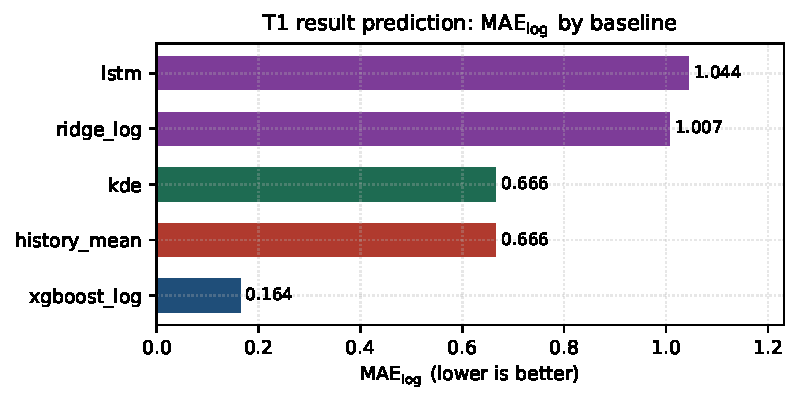
\includegraphics[width=\linewidth]{figures/fig2_result_prediction.pdf}
    \caption{\task{1} \maelog{}.}
    \label{fig:t1}
  \end{subfigure}\hfill
  \begin{subfigure}[b]{0.32\linewidth}
    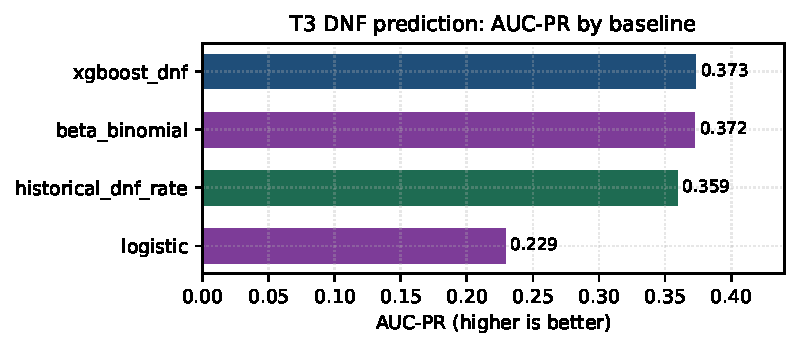
\includegraphics[width=\linewidth]{figures/fig3_dnf_models.pdf}
    \caption{\task{3} \aucpr{}.}
    \label{fig:t3}
  \end{subfigure}\hfill
  \begin{subfigure}[b]{0.32\linewidth}
    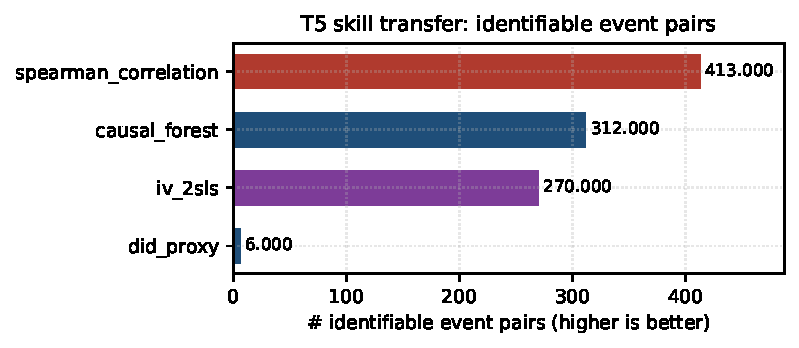
\includegraphics[width=\linewidth]{figures/fig4_transfer_pairs.pdf}
    \caption{\task{5} pairs.}
    \label{fig:t5}
  \end{subfigure}
  \caption{Per-task detail for \task{1}, \task{3} and \task{5}.}
  \label{fig:taskdetail}
\end{figure}

\subsection{Reproducing these numbers}
\label{sec:results-repro}

All numbers above are regenerated by the released pipeline:
\begin{center}\small
\code{build\_dataset} $\to$
\code{run\_all\_baselines --mode small --device cuda} $\to$
\code{run\_multi\_seed --seeds 42 43 44 --mode small --device cuda} $\to$
\code{build\_leaderboard}.
\end{center}
The offline path substitutes a synthetic generator so that continuous
integration runs without network access; results computed on synthetic data are
labelled as such and never enter the leaderboard. Each baseline writes a
structured report containing overall metrics, the four stratified views,
calibration, significance tests against the registered reference baselines and
a cost file (with device and GPU/CPU hours), exactly as specified in
Section~\ref{sec:protocol}.

\section{Discussion}
\label{sec:discussion}

\subsection{What the baselines tell us}
\label{sec:disc-insights}

The measured results support four methodological observations.

\paragraph{Simple, well-specified models are strong.} On \task{2}, the official
psychology sheet, a Plackett--Luce model and a kernel-density simulation all
produce identical Kendall $\kendall=0.7673$ in the seed-42 run and
$0.8132\pm0.0342$ across seeds. On \task{3}, the historical \DNF{} rate
($0.3591$) is statistically indistinguishable from the best tree model
($0.3731$, $p=0.749$, negligible effect), and a Bayesian Beta--Binomial
posterior ($0.3725$) is in fact best \emph{on average} across seeds
($0.2938\pm0.0570$ vs $0.2779\pm0.0724$ for the tree model). In both cases a
simple, domain-informed baseline matches or nearly matches more expressive
alternatives. This is not a reason to abandon richer models; it is a calibration
of expectations. A benchmark that reports only ``model A beats model B'' hides
the fact that both may be matched by a good prior at a fraction of the cost.

\paragraph{Generic deep and graph models underperform here.} Two of the six
methodological families do markedly worse than their simpler counterparts, and
the multi-seed results make the gap robust to evaluation-set resampling. On
\task{1}, the LSTM (\maelog{} $=1.0440$, or $0.9436\pm0.0754$ across seeds) is
the \emph{worst} baseline, worse even than the historical mean
($0.6657$), with a large paired effect against the tree model
($\Delta=+1.087$, $p=5.2\times10^{-8}$, Cohen's $d=0.90$). On \task{2}, the GNN
($\kendall=0.5670$, or $0.7440\pm0.1258$ across seeds) trails the psychology
sheet by $0.200$ ($p=3.2\times10^{-7}$, $d=0.56$). Meanwhile rule-aware
features plus tree boosting win \task{1} and are competitive on \task{3}. At
this sample size and feature budget, the domain structure---competitor history,
round format, event identity---appears to matter more than architectural
capacity, and sequence and graph models likely need domain-specific inductive
biases before they can compete. We regard this as the benchmark's clearest
actionable finding.

\paragraph{The hard cases are structural, not incidental.} Errors concentrate
where the data are thin or the phenomenon is stochastic: novices on \task{1}
(\maelog{} $0.4151$), the late test slice on \task{2} ($\kendall=0.6437$) and
\task{3} (\aucpr{} $0.2962$), elites on \task{3} (\aucpr{} $0.1399$), and
cold-start competitors everywhere (\maelog{} $0.9827$). These are not sampling
accidents; they follow from little history, distribution shift and
near-deterministic execution. A useful benchmark must therefore be judged on
the hard subsets, which is why \wcabench{} makes them first-class.

\paragraph{Extrapolation and identification are where claims become fragile.}
\task{4} and \task{5} are included precisely because they are hard to validate.
The \task{4} three-by-three estimates span $3.02$~s (change point), $3.29$~s
(GP+EVT) and $3.74$~s (exponential decay), all far from the community anchor of
$\approx 2.37$~s. None is ``wrong'' in a statistical sense---each is a
consistent fit to its assumptions---but the spread across reasonable methods is
itself the finding, and the aggregate stability scores are not significantly
separated at $21$ events. Similarly, the number of transfer pairs identified
drops from $413$ (correlation) to $312$ (causal forest) to $270$ (IV) to $6$
(DID; $2$ on average across seeds). Reporting the disagreement and the
non-identifiability, rather than a single number, is the scientifically honest
outcome.

\paragraph{Evaluation-set variance matters.} Re-running over three seeds shows
that some conclusions are stable (the tree model wins \task{1} by a wide margin
under every seed) while others are not (the \task{3} winner flips between the
tree model and the Beta--Binomial prior, and the GNN's \task{2} spread,
$\pm0.1258$, is larger than several inter-model gaps). Single-run leaderboards
in this domain should therefore be read with the multi-seed table alongside
them.

\subsection{Towards avoiding saturation}
\label{sec:disc-saturation}

Benchmarks decay: once a task is solved, it stops discriminating. We built two
defences. First, the five tasks form a difficulty spectrum from well-specified
regression to causal identification, so improvements at the easy end do not
exhaust the benchmark. Second, every task carries a hard subset
(Section~\ref{sec:protocol-stratification}); for \task{3}, restricting to
competitors with a historical \DNF{} rate in $[0.1,0.3]$ removes the
easy-to-classify extremes, and for \task{2} the near-tie subset removes rounds
where ranking is trivial. The small-mode results already show that several
subsets are far from saturated, for example elite \task{3} (\aucpr{}
$0.1399$) and cold-start \task{1} (\maelog{} $0.9827$), so the benchmark retains
headroom.

\subsection{Why a domain benchmark, and why speedcubing}
\label{sec:disc-domain}

The coexistence of strong simple models and more expressive alternatives
recalls the long-standing tension between data modelling and algorithmic
prediction \citep{breiman_cultures}: the benchmark's job is to make the
comparison fair, not to anoint a winner. \wcabench{} is a case study in a
broader idea: \emph{rule-governed individual sports} are an underused testbed
for machine learning. Such data combine large scale with genuine
structure---explicit formats, deterministic averaging rules, discrete status
codes---that is invisible to generic pipelines but decisive for accuracy.
Speedcubing is an unusually clean instance: it is fully individual, precisely
timed to the centisecond, globally distributed and publicly released. The
lessons transfer to swimming, track and field, or powerlifting, where analogous
round formats and disqualification rules exist. We therefore see \wcabench{}
less as an endpoint than as a template for building trustworthy benchmarks in
rule-governed athletic domains.

\subsection{Open problems}
\label{sec:disc-open}

Several directions are deliberately left open. Sequence models
(LSTM/Transformer) and graph neural networks currently underperform, so the open
question is not whether they are more accurate in principle but what
domain-specific inductive biases---event-aware embeddings, round-format
constraints, or interaction graphs anchored on head-to-head history---would let
them exploit the structure that tree models already capture. On \task{5}, the
steep drop from $413$ correlational pairs to $270$ IV pairs and $6$ DID pairs
invites more credible causal designs (for example instruments built from the
staggered domestic introduction of events, or synthetic-control designs) while
the difficulty of validating any of them motivates better sensitivity analysis.
Finally, the interaction between non-stationarity and event scale suggests that
per-event hierarchical normalization, rather than a single global
preprocessing, may be the most promising generic improvement.

\section{Limitations}
\label{sec:limitations}

We are explicit about what \wcabench{} cannot support, because a benchmark's
credibility depends on the honesty of its caveats.

\paragraph{Extrapolation risk (\task{4}).} Human-limit estimation has no
observable ground truth and is intrinsically vulnerable to structural change.
Historical data cannot anticipate a future jump driven by new hardware (for
example magnetic cubes), new training regimes, or rule changes. The
discrepancy between the three-by-three estimates of the change-point model
($3.02$~s), the Gaussian-process/extreme-value model ($3.29$~s) and exponential
decay ($3.74$~s), and the community anchor ($\approx 2.37$~s), should be read as
a warning, not as a resolution. Limits reported here are model-conditional
statements, not facts about human ability.

\paragraph{Regional imbalance.} Access to sanctioned competitions is uneven
across countries and continents. Because features such as competition count and
opponent strength are partly proxies for opportunity, cross-regional
generalization claims are weak. We report continental strata for transparency,
but small strata (for example Oceania, South America) contain too few test
instances for reliable conclusions, and several stratified cells are
undefined.

\paragraph{Self-selection and confounding (\task{5}).} Participation in an
event is a choice correlated with ability. Correlation-based transfer
estimates therefore overstate effects, and even the DID proxy relies on a
parallel-trends assumption that self-selection may violate. The
``identifiable pair count'' is a measure of how much the data support an
estimate, not a guarantee of a causal effect. \wcabench{} should not be used to
make causal claims about training without an explicit identification argument.

\paragraph{Temporal non-stationarity.} The training window (2003--2022) differs
from the test window (2025--2026) in hardware, rules and participant
demographics. Models may degrade in ways that reflect genuine distribution
shift rather than modelling error; the falling \task{2} Kendall $\kendall$
across test slices ($0.90 \to 0.64$) is consistent with exactly this.

\paragraph{Sampled small-mode results.} The headlines in
Section~\ref{sec:results} come from a sampled test window run on a single
machine with one GPU (Section~\ref{sec:compute}). Absolute values will move
when the full rolling-window protocol is executed on all $1{,}719{,}290$ test
records, and ranking ties (such as the \task{2} $0.7673$ tie) may resolve
differently; the three-seed table (Section~\ref{sec:results-multiseed}) is
included precisely to expose this sampling variance but does not substitute for
the full run. We report the sampled numbers because they are real and
verifiable, not because they are final; the released pipeline supports the full
run.

\paragraph{Imbalanced, sparse classes.} \DNF{} prediction and skill-transfer
estimation both suffer from severe imbalance and sparsity. Even conditioning on
rounds that reach the decision point, the positive rate varies from single
digits in some events to about $95\%$ in three-by-three blindfolded, and many
event pairs have too few common competitors for stable estimation.

\paragraph{Native backends and compute reproducibility.} This release runs the
tree baselines on native XGBoost and the GNN on its native CUDA path
(Section~\ref{sec:compute}); every report records the device, wall-clock time
and CPU/GPU hours actually used. Readers reproducing a baseline should hold the
library versions and device fixed: a different backend (for example a
scikit-learn fallback for the tree models, or a CPU-only graph kernel) will not
reproduce these numbers exactly, and the earlier fallback-backed results
differed materially from the native ones.

\paragraph{Single-snapshot data.} Even with a fixed export (v2.0.2), the \wca{}
occasionally corrects historical results, and the database grows continuously:
each weekly export carries a new sequential version label and additional
competitions. We pin the 2026-09-21 snapshot and record it, so the exact scale
figures (for example $6{,}909{,}454$ results) are snapshot-specific and a newer
export will show slightly larger numbers. Readers comparing against the current
official download should treat our counts as a frozen baseline rather than a
live value.

\section{Ethics and Broader Impact}
\label{sec:ethics}

\paragraph{Permitted uses.} \wcabench{} is intended for scientific research and
teaching: sports data analysis, benchmark methodology, and reproducible
evaluation of prediction and inference methods. It may also serve the
speedcubing community directly, for example to help competitors understand
their own progression or organisers to reason about round structure.

\paragraph{Prohibited uses.} The accompanying data card forbids, in the
strongest terms, the use of these data or models for:
\begin{itemize}
  \item \textbf{gambling, betting or wagering} of any kind, including
        predictive services marketed to bettors;
  \item \textbf{discriminatory screening, profiling or shaming} of individual
        competitors;
  \item \textbf{impersonating} the \wca{} or other official bodies, or
        fabricating competition results; and
  \item redistributing individual-level derived data without anonymization.
\end{itemize}
These prohibitions are not decorative. Aggregate competition records are
public, but they are records of identifiable people, and their aggregation
enables inference that individuals did not consent to. The risk that a
predictive benchmark is repurposed for betting is real enough that we treat its
prevention as a design requirement.

\paragraph{Attribution.} All derived publications must carry the \wca{}
attribution notice: “This information is based on competition results owned and
maintained by the World Cube Association, published at
\url{https://worldcubeassociation.org/results}.” Code is released under
Apache-2.0; data rights remain with the \wca{}.

\paragraph{Privacy and opt-out.} Although the underlying data are public,
individuals may have legitimate reasons to withdraw. We therefore commit to an
opt-out mechanism: a competitor may contact the maintainers to request removal
of their individual-level derived features from released artifacts. Aggregate
statistics---which do not single out an individual---are retained, so the
benchmark's scientific claims remain reproducible while the individual's
choice is respected. We also recommend that challenge organisers restate the
prohibited uses in their rules and that the \wca{} Results Team remain a
standing point of contact.

\paragraph{Fairness considerations.} Because regional opportunity is unequal,
a model trained predominantly on data from well-represented regions may perform
worse for under-represented ones, and this could, if misused, disadvantage
competitors from those regions. We mitigate by stratifying by continent and by
refusing to publish individual-level rankings as products. We do not claim that
stratification resolves the underlying inequity; it only makes it visible.

\paragraph{Broader impact.} We hope \wcabench{} nudges sports machine learning
towards more rigorous evaluation: time-aware splits, frozen statistics,
stratified reporting, effect sizes and explicit identification assumptions.
The main societal risk is misuse for betting or individual targeting, which the
data card and the opt-out mechanism are designed to discourage.

\section{Conclusion}
\label{sec:conclusion}

We presented \wcabench, a standardized benchmark for prediction and inference
on World Cube Association competition data. Built on an official export of
$6{,}909{,}454$ results spanning $298{,}551$ competitors and $18{,}708$
competitions, it formalizes five tasks---result prediction, placement
prediction, \DNF{} prediction, human-limit estimation and skill
transfer---under a single interface with a leakage-safe rolling-window
protocol, frozen statistics, four-dimensional stratification, a full
statistical-testing toolbox with effect sizes, and a documented compute and
hardware specification.

Beyond the infrastructure, the paper reports 21 real reference baselines across
six methodological families, each evaluated both for a single seed and as a
mean over three seeds. These include a strong tree-based result model
(\maelog{} $=0.164$, or $0.1055\pm0.0417$ across seeds) that beats a sequence
model by roughly an order of magnitude, a three-way Kendall $\kendall=0.7673$
placement tie among the psychology sheet, Plackett--Luce and a kernel-density
simulation while a graph network reaches only $0.567$, a tree-based \DNF{}
classifier (\aucpr{} $=0.373$) whose edge over the historical rate is \emph{not}
significant and which is beaten on average by a simple Beta--Binomial prior,
event-level human-limit estimates that disagree sharply with domain anchors,
and a monotone collapse in identified transfer pairs from $413$ (correlation)
to $6$ (difference-in-differences). We deliberately frame these as a
reproducible starting point rather than as state-of-the-art claims.

The benchmark's value is the question it makes answerable: under the real
constraints of a rule-governed sport, how do different methodological families
compare? We release the data pipeline, task definitions, baseline
implementations and leaderboard tooling, and we invite the community to improve
the baselines and to extend the tasks. Future work includes full-scale
rolling-window evaluation on all $1.72$M test records across many seeds,
domain-aware sequence and graph baselines that can exploit round-format and
head-to-head structure, genuinely causal designs for \task{5}, and a community
challenge with a public leaderboard. We hope \wcabench{} both serves
speedcubing and offers a reusable template for trustworthy benchmarking in
other rule-governed athletic domains.


% ------------------------------------------------------------ bibliographies
\bibliographystyle{plainnat}
\bibliography{references}

% ----------------------------------------------------------------- appendix
\appendix
\section{Task metric reference}
\label{app:metrics}

Table~\ref{tab:metric-ref} collects every metric required per task, its
direction and the reason it is included. This is the normative list that a
submission's report must contain.

\begin{table}[h]
  \centering
  \small
  \begin{threeparttable}
  \caption{Normative metric list per task. ``Dir.'' indicates the preferred
  direction of the primary metric.}
  \label{tab:metric-ref}
  \begin{tabular}{@{}llll@{}}
    \toprule
    Task & Metric & Dir. & Notes \\
    \midrule
    \task{1} & \maelog{} & $\downarrow$ & primary; log domain \\
    \task{1} & \rmselog{} & $\downarrow$ & sensitive to outliers \\
    \task{1} & interval coverage & $\to 0.90$ & calibration of 90\% intervals \\
    \midrule
    \task{2} & Kendall $\kendall$ & $\uparrow$ & primary rank correlation \\
    \task{2} & top-3 overlap & $\uparrow$ & podium accuracy \\
    \task{2} & Brier (podium) & $\downarrow$ & probabilistic ranking quality \\
    \midrule
    \task{3} & \aucpr{} & $\uparrow$ & primary under imbalance \\
    \task{3} & \aucroc{} & $\uparrow$ & reported but not primary \\
    \task{3} & F1, MCC & $\uparrow$ & thresholded performance \\
    \task{3} & calibration error & $\downarrow$ & reliability diagram \\
    \midrule
    \task{4} & LOO stability (std) & $\downarrow$ & leave-one-out refit variance \\
    \task{4} & interval coverage & $\to$ nominal & predictive calibration \\
    \task{4} & domain consistency & qualitative & vs.\ expert anchors \\
    \midrule
    \task{5} & point-estimate accuracy & $\uparrow$ & vs.\ held-out data \\
    \task{5} & subsample robustness & $\uparrow$ & stability across subsets \\
    \task{5} & \# identifiable pairs & --- & honesty about support \\
    \bottomrule
  \end{tabular}
  \end{threeparttable}
\end{table}

\section{Worked examples for the multi-blind encoding}
\label{app:multi}

We give two round-trip examples, one per encoding generation, that the test
suite asserts.

\paragraph{Old format \texttt{1SSAATTTTT}.} Let solved $=5$, attempted $=6$,
time $=300$~s. Then missed $=1$, $SS = 99-5 = 94$, $AA = 06$, and the stored
integer is
$1\!\times\!10^{9} + 94\!\times\!10^{7} + 6\!\times\!10^{5} + 300
= 1{,}940{,}600{,}300$.
Decoding recovers $SS=94$, $AA=06$, seconds $=300$, hence solved $=99-94=5$,
attempted $=6$, missed $=1$.

\paragraph{New format \texttt{0DDTTTTTMM}.} Let solved $=10$, attempted $=12$,
missed $=2$, time $=600$~s. Then difference $=10-2=8$, $DD = 99-8 = 91$,
$MM = 02$, and the stored integer is
$91\!\times\!10^{7} + 600\!\times\!100 + 2 = 910{,}060{,}002$, i.e.\ the
zero-padded string \code{0910060002}. Decoding gives $DD=91$, seconds $=600$,
$MM=02$, difference $=8$, solved $=8+2=10$, attempted $=12$.

The encoder rejects impossible values (attempted $>99$, time $>99{,}999$~s,
or a negative difference in the new format), and the decoder rejects negative
or out-of-range integers. A round-trip test
$\mathrm{encode}(\mathrm{decode}(v)) = v$ is part of the continuous-integration
gate.

\section{Scale-robust view of \task{4} limits}
\label{app:limit}

The aggregate \task{4} stability statistic is dominated by the multi-blind
event, whose encoded limit is of order $10^{8}$ and which therefore dwarfs the
centisecond-scale events in any unweighted mean. Table~\ref{tab:limit} reports
per-event limits for a representative subset, comparing the most stable method
(\texttt{gp\_evt}) with exponential decay, so that the numbers can be read on a
human scale. Values are the fitted asymptotes $L$ of Equation~\ref{eq:limit};
$n$ is the number of world-record points used by the stability estimate.

\begin{table}[h]
  \centering
  \small
  \begin{threeparttable}
  \caption{Human-limit estimates for selected events: \texttt{gp\_evt}
  (Gaussian process $+$ extreme-value theory) versus exponential decay.
  $L$ in seconds unless noted; the underlying solver stores centiseconds.}
  \label{tab:limit}
  \begin{tabular}{@{}lrrr@{}}
    \toprule
    Event & \texttt{gp\_evt} $L$ (s) & \texttt{exp\_decay} $L$ (s) & $n$ \\
    \midrule
    \code{222} (2$\times$2) & 0.32 & 0.52 & 16 \\
    \code{333} (3$\times$3) & 3.29 & 3.74 & 26 \\
    \code{333oh} (one-handed) & 4.67 & 6.82 & 25 \\
    \code{444} (4$\times$4) & 10.18 & 17.09 & 33 \\
    \code{555} (5$\times$5) & 26.95 & 35.08 & 28 \\
    \code{666} (6$\times$6) & 45.73 & 51.35 & 19 \\
    \code{777} (7$\times$7) & 78.73 & 110.31 & 18 \\
    \code{pyram} (pyraminx) & 0.40 & 1.04 & 15 \\
    \code{skewb} & 0.45 & 0.75 & 17 \\
    \code{sq1} (square-1) & 2.08 & 4.43 & 24 \\
    \code{333fm} (fewest moves) & 14.42 (moves) & 7.70 (moves) & 9 \\
    \bottomrule
  \end{tabular}
  \begin{tablenotes}\footnotesize
    \item The three-by-three estimates span $3.02$~s (change point), $3.29$~s
          (\texttt{gp\_evt}) and $3.74$~s (exponential decay), all above the
          community anchor of $\approx 2.37$~s. The multi-blind event
          (\texttt{gp\_evt} limit $\sim 4.8\times 10^{8}$ in encoded units) is
          excluded from this table.
  \end{tablenotes}
  \end{threeparttable}
\end{table}

\section{Reproduction artifacts}
\label{app:artifacts}

Table~\ref{tab:artifacts} lists the released components that support
reproduction, and the commands that rebuild them.

\begin{table}[h]
  \centering
  \small
  \begin{threeparttable}
  \caption{Released artifacts and their rebuild commands.}
  \label{tab:artifacts}
  \begin{tabular}{@{}ll@{}}
    \toprule
    Artifact & Command / location \\
    \midrule
    Processed Parquet tables & \code{build\_dataset --source raw} \\
    Temporal split indices & produced by the dataset build \\
    Frozen person--event statistics & produced by the dataset build (612{,}224 rows) \\
    Baseline results & \code{run\_all\_baselines --mode small} \\
    Leaderboard & \code{build\_leaderboard} \\
    Synthetic CI data & \code{generate\_synthetic --small} \\
    Data card & repository root \code{datacard.md} \\
    \bottomrule
  \end{tabular}
  \end{threeparttable}
\end{table}

\paragraph{Submission format.} A leaderboard submission contains a report
directory (overall, by-event, by-skill-level, by-time-slice, by-continent,
calibration, significance and cost files), the raw per-instance predictions, a
model/training configuration, an environment lock file, the seed list and a
README. The minimum accepted reproducibility level is L2; the main leaderboard
requires L3 (Section~\ref{sec:protocol-repro}).

\paragraph{Citation and license.} Code is released under Apache-2.0. Any
derived work must reproduce the \wca{} attribution notice given in
Section~\ref{sec:ethics}.


\end{document}
